\documentclass[a4paper]{article}

\usepackage[utf8]{inputenc}
\usepackage[portuguese]{babel}
\usepackage{a4wide}
\usepackage[pdftex]{hyperref}
\usepackage{graphicx}
\graphicspath{ {imagens/} } % path de imagens começa nesta pasta
\usepackage{wrapfig}
\usepackage{caption}
\usepackage{float}
\usepackage{amsmath}
\usepackage{subcaption}
\usepackage{tikz}
\usepackage{placeins}
\usetikzlibrary{patterns}

%%%%%%%%%%%%%%%%%% SQL STYLE %%%%%%%%%%%%%%%%

\usepackage{xcolor,listings}
\usepackage{textcomp}
\usepackage{color}

\definecolor{codegreen}{rgb}{0,0.6,0}
\definecolor{codegray}{rgb}{0.5,0.5,0.5}
\definecolor{codepurple}{HTML}{C42043}
\definecolor{backcolour}{HTML}{F2F2F2}
\definecolor{bookColor}{cmyk}{0,0,0,0.90}  
\color{bookColor}

\lstset{upquote=true}

\lstdefinestyle{SQL}{   language=SQL,
    commentstyle=\color{codegreen},
    keywordstyle=\color{codepurple},
    numberstyle=\numberstyle,
    stringstyle=\color{codepurple},
    basicstyle=\footnotesize\ttfamily,
    breakatwhitespace=false,
    breaklines=true,
    captionpos=b,
    keepspaces=true,
    numbers=left,
    numbersep=10pt,
    showspaces=false,
    showstringspaces=false,
    showtabs=false,
}

\newcommand\numberstyle[1]{%
    \footnotesize
    \color{codegray}%
    \ttfamily
    \ifnum#1<10 0\fi#1 |%
}


%%%%%%%%%%%%%%%%%% JAVA STYLE %%%%%%%%%%%%%%%%

\definecolor{javaorange}{rgb}{0.9,0.6,0.4} % for keywords
\definecolor{javagreen}{rgb}{0.45,0.75,0.55} % comments
\definecolor{javablue}{rgb}{0.3,0.45,0.75} % strings
\definecolor{javadocblue}{rgb}{0.25,0.35,0.75} % javadoc
 
\lstdefinestyle{JAVA}{language=Java,
basicstyle=\ttfamily,
keywordstyle=\color{javaorange},
stringstyle=\color{javablue},
commentstyle=\color{javagreen},
morecomment=[s][\color{javadocblue}]{/**}{*/},
tabsize=4,
showspaces=false,
showstringspaces=false,
breaklines=true}

%%%%%%%%%%%%%%%%%%%%%%%%%%%%%%%%%%%%%%%%%%%%%%


% Fonte de jeito! Times New Roman <3
\usepackage{times}

\newcommand{\question}[1]{\textcolor{gray}{\textit{"#1"}}} % style para questões

\begin{document}

\begin{titlepage}
\begin{center}


\includegraphics[width=0.6\textwidth]{capa/logo.jpg}\\[.75cm]

\textsc{\LARGE Universidade do Minho}\\[0.7cm] % Name of your university/college
\textsc{\Large Departamento de Informática}\\[0.7cm] % Major heading such as course name
\textsc{\large Administração e Exploração de Base de Dados}\\[0.7cm] % Minor heading such as course title]

% Title
\rule{\linewidth}{0.5mm} \\[0.5cm]
{ \huge \bfseries Monitor de uma Base de Dados Oracle\\[0.5cm] }
\rule{\linewidth}{0.5mm}\\[0.7cm]

% Date
{\Large \today}\\[1cm] % Date, change the \today to a set date if you want to be precise

% Author and supervisor
\emph{\Large \textbf{GRUPO 2:} }\\[0.6cm]

\noindent
\begin{minipage}{0.26\textwidth}
    Francisco Matos\\ \textsc{(A77688)}\\
    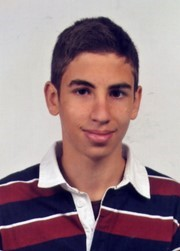
\includegraphics[height = 4cm, width=3.7cm]{capa/FranciscoMatos.jpg}\break
\end{minipage}%
\begin{minipage}{0.26\textwidth}
    Francisco Oliveira\\ \textsc{(A78416)}\\
    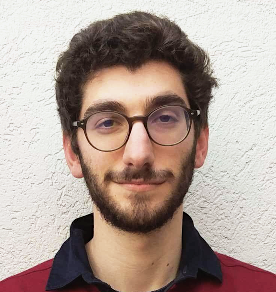
\includegraphics[height = 4cm, width=3.7cm]{capa/kiko.png}\break
\end{minipage}%
\begin{minipage}{0.26\textwidth}
    Gil Cunha\\ \textsc{(A77249)}\\
    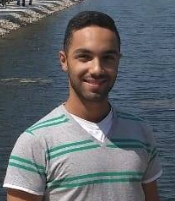
\includegraphics[height = 4cm, width=3.7cm]{capa/gil.png}\break
\end{minipage}%
\begin{minipage}{0.26\textwidth}
    Luís Costa\\ \textsc{(A74819)}\\
    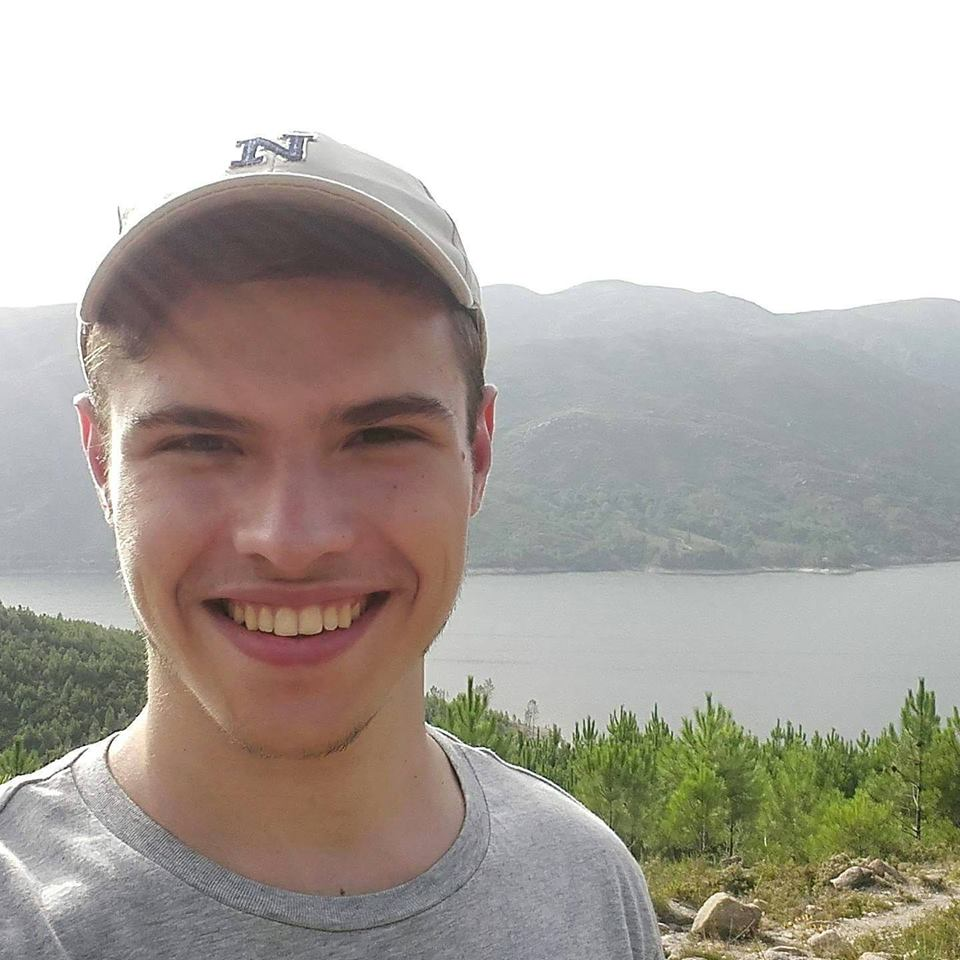
\includegraphics[height = 4cm, width=3.7cm]{capa/luis.jpg}\break
\end{minipage}%

\vfill


\end{center}
\end{titlepage}

\pagebreak
\tableofcontents
\newpage

\section{Introdução}
\hspace{3mm} 

Neste trabalho será apresentada a criação de um monitor básico que permita a visualização, de forma simples, dos principais parâmetros de avaliação de \emph{performance} de uma BD \emph{Oracle}.

Para tal desenvolveu-se um agente de recolha de informação em Java, que através de \emph{Views} de administração, obtém os dados necessários e armazena-os num \emph{Schema} em \emph{Oracle} previamente criado.

Finalmente, usando uma API em \emph{REST}, ativou-se este serviço na Base de Dados do Monitor e devolve-os em JSON, possibilitando uma apresentação mais intuitiva numa interface \emph{web} em HTML5.

\newpage


\section{Base de Dados}
\hspace{3mm} 

Neste trabalho prático, o grupo decidiu criar um monitor direcionado à \textbf{Base de Dados Pluggable \emph{orcl}}.
Para iniciar este projeto considerou-se importante, em primeiro lugar, a necessidade do planeamento ao nível da base de dados \emph{Oracle} a ser utilizada pelo monitor, para armazenamento de informação e gestão. Algo a ter em conta foram os \emph{users} que teríamos de utilizar para aceder à base de dados a monitorizar, e as suas permissões. \\

Através do esquema seguinte, podemos concluir que existem vários utilizadores, com permissões diferentes entre si:

\begin{itemize}
    \item \textit{\textbf{sys.cdb:}} utilizador administrador da \emph{CDB (Container Database)}, que consegue aceder e gerir todos os dados da base de dados geral (\emph{root}); 
    
    \item \textit{\textbf{sys.orcl:}} utilizador administrador da \emph{PDB orcl (Pluggable Database)}, que consegue aceder e gerir os dados da PDB respetiva; 
    
    \item \textit{\textbf{hr.orcl \& grupo2.orcl:}} utilizadores comuns da \emph{PDB (Pluggable Database)}. O \textbf{grupo2} será o utilizador formado pelo grupo do projeto para criar e gerir a base de dados para o monitor final. Este será descrito na secção \ref{users} - \textbf{Utilizadores} deste documento; 
\end{itemize}

\begin{figure}[H]
\centering
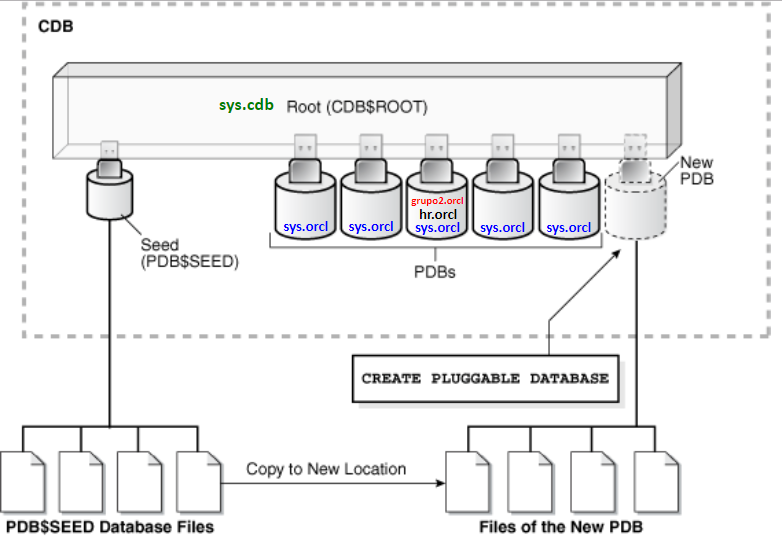
\includegraphics[scale=0.8]{arquitetura.png}
\caption{Arquitetura geral do sistema ORACLE DB - \textbf{ PDB orcl} contêm utilizadores \emph{sys, hr e grupo2}}
\end{figure}

\newpage
\subsection{Modelo Conceptual}
\hspace{3mm} 
O modelo conceptual desenvolvido teve por base as \emph{views} disponíveis nos utilizadores \emph{sys}, sobre a BD em questão, e as informações que o grupo considerou relevante recolher para monitorizar a base de dados. Estas \emph{views} serão descritas em pormenor na secção de \ref{ligacaoBD} - \textbf{Ligação à Base de Dados}. O resultado passou então numa análise prévia dos atributos das respetivas \emph{views} e da informação que estas tabelas permitiam extrair. No final, concluiu-se as seguintes entidades:
\textbf{DB, CPU, Memory, Tablespace, Datafile, User e Role.} Os respetivos atributos são explicados na secção seguinte.

O modelo conceptual desenhado apresenta-se de seguida:

\begin{figure}[H]
\centering
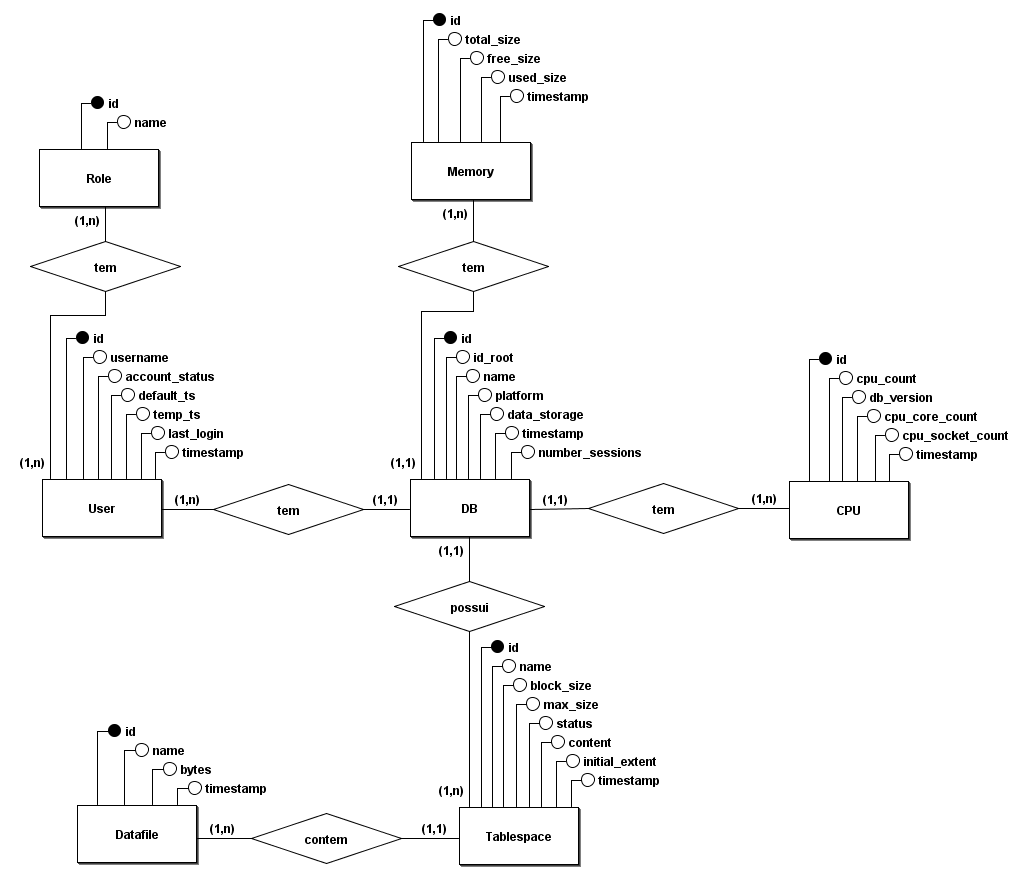
\includegraphics[scale=0.45]{modelo_conceptual.png}
\caption{Modelo Conceptual da Base de Dados do Monitor}
\end{figure}

\newpage

\subsection{Análise de Entidades \& Atributos}
De forma a ter um melhor entendimento do significado das entidades e seus atributos e sobre aquilo que representam, o grupo desenvolveu tabelas que os descrevem detalhadamente:\\

A entidade \textbf{DB}, referente à base de dados \emph{pluggable orcl} a analisar, possui \textbf{id\_db, id\_db\_root, name, platform, data\_storage, number\_sessions e db\_timestamp.}

\begin{figure}[H]
\centering
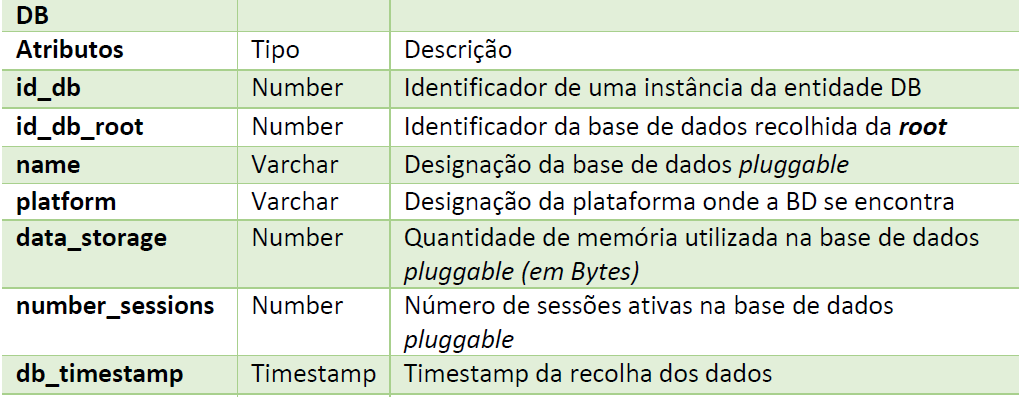
\includegraphics[scale=0.65]{db.PNG}
\caption{Informação de DB}
\end{figure}

A entidade \textbf{CPU}, referente ao cpu da base de dados \emph{Pluggable orcl}, possui \textbf{id\_cpu, db\_version, cpu\_count, cpu\_core\_count, cpu\_socket\_count e cpu\_timestamp.}

\begin{figure}[H]
\centering
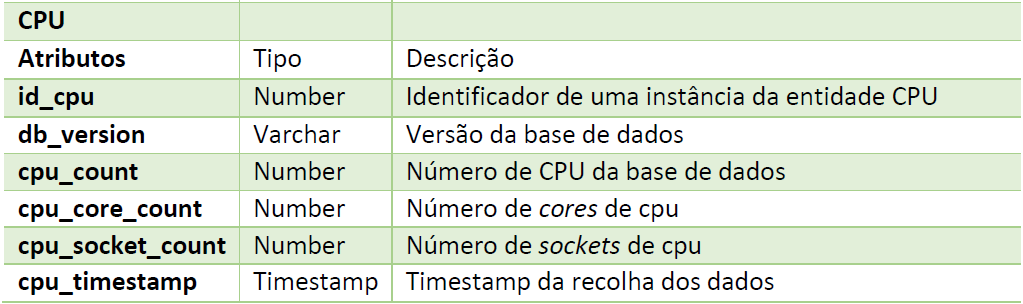
\includegraphics[scale=0.65]{cpu.PNG}
\caption{Informação de CPU}
\end{figure}

Quanto à Memória, foi necessário um estudo prévio da estrutura básica da memória da base de dados Oracle \footnote{https://docs.oracle.com/database/121/CNCPT/memory.htm#CNCPT7777}.

A base de dados Oracle possui várias áreas de memória, em que cada uma contem vários componentes. Sendo assim, o grupo focou em apenas duas das estruturas básicas da memória da BD \emph{Oracle}:

\begin{itemize}
    \item \emph{\textbf{System Global Area (SGA):}} O SGA é um grupo de componentes de memória partilhada, que contêm dados e informação de controlo para uma instância da base de dados \emph{Oracle}. Todos os servidores e processos em \emph{background} partilham o SGA. 
    
    \item \emph{\textbf{Program Global Area (PGA):}} O PGA é uma região de memória não partilhada que contém dados e informação de controlo exclusivamente para o uso de um processo Oracle. A base de dados \emph{Oracle} cria um PGA diferente, de cada vez que um processo \emph{Oracle} se inicia.
\end{itemize}

Visto estas definições, o grupo considerou mais interessante monitorizar a memória da Base de Dados \emph{Oracle}, servindo-se da informação das \emph{views} disponíveis sobre a memória, relativas ao \textbf{SGA}.\\

A entidade \textbf{Memory} possui os atributos \textbf{id\_mem, total\_size\_mb, free\_size\_mb, used\_size\_mb e mem\_timestamp.}

\begin{figure}[H]
\centering
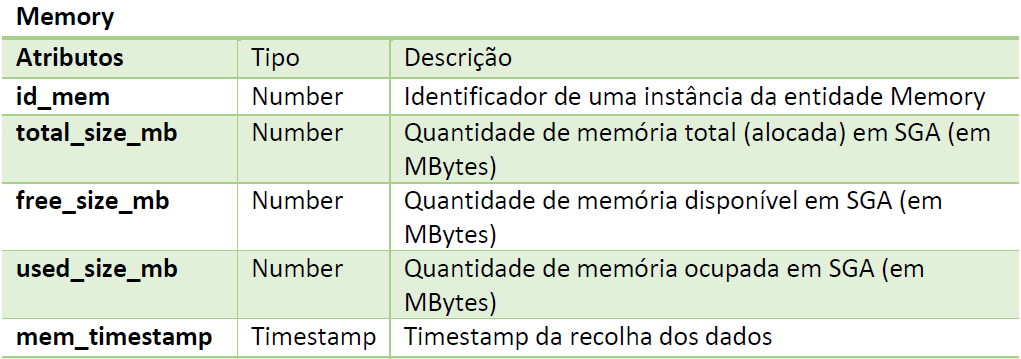
\includegraphics[scale=0.65]{memory.PNG}
\caption{Informação da Memory}
\end{figure}

A entidade \textbf{Tablespace} representa cada uma das \emph{tablespaces} associadas à BD \emph{Pluggable}, e possui \textbf{id\_tablespace, name, block\_size, max\_size, status, contents, initial\_extent e ts\_timestamp.}

\begin{figure}[H]
\centering
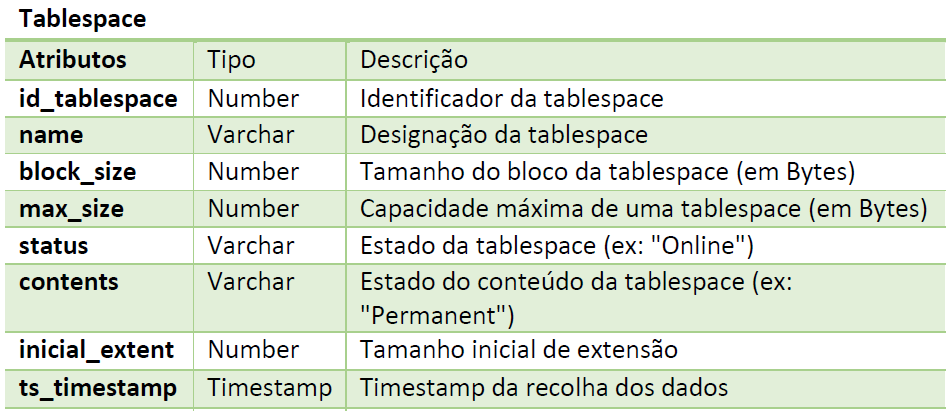
\includegraphics[scale=0.65]{tablespace.PNG}
\caption{Informação de Tablespace}
\end{figure}

A entidade \textbf{Datafile} representa cada \emph{datafile} associado a cada uma das \emph{tablespaces} que a BD \emph{Pluggable} contém, e possui \textbf{id\_datafile, name, bytes e df\_timestamp}.

\begin{figure}[H]
\centering
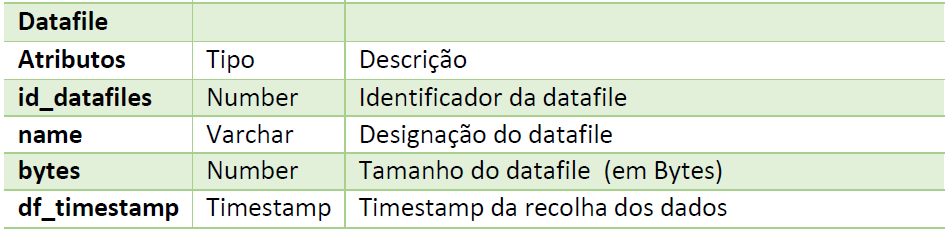
\includegraphics[scale=0.65]{datafile.PNG}
\caption{Informação de Datafile}
\end{figure}

\newpage

A entidade \textbf{User} representa os utilizadores da BD \emph{Oracle} e possui \textbf{id\_user, username, account\_status, default\_ts, temp\_ts, last\_login e user\_timestamp.}

\begin{figure}[H]
\centering
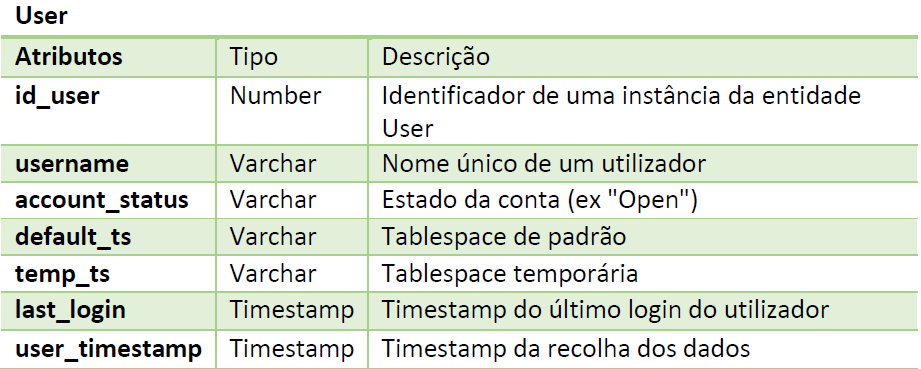
\includegraphics[scale=0.65]{user.PNG}
\caption{Informação de User}
\end{figure}

A entidade \textbf{Role} representa todos os papeis/funções (\emph{roles}) que um utilizador pode possuir na BD \emph{Oracle}. Este é um conjunto de privilégios que se pode conceder a um \emph{user} e possui \textbf{id\_role} e \emph{name}.

\begin{figure}[H]
\centering
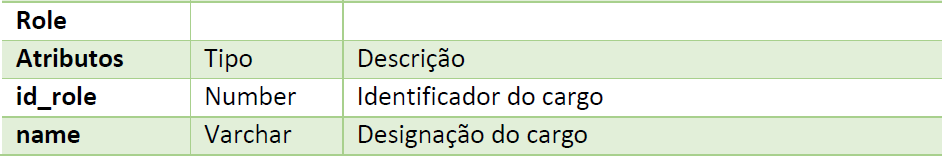
\includegraphics[scale=0.65]{role.PNG}
\caption{Informação de Role}
\end{figure}


\newpage
\subsection{Modelo Lógico}
\hspace{3mm} 

De acordo com o Modelo Conceptual foi possível proceder a realização do Modelo Lógico, tendo em especial atenção às restrições das chaves primárias e estrangeiras de cada tabela e à relação N-N presente na base de dados. O modelo lógico apresenta-se de seguida:

\begin{figure}[H]
\centering
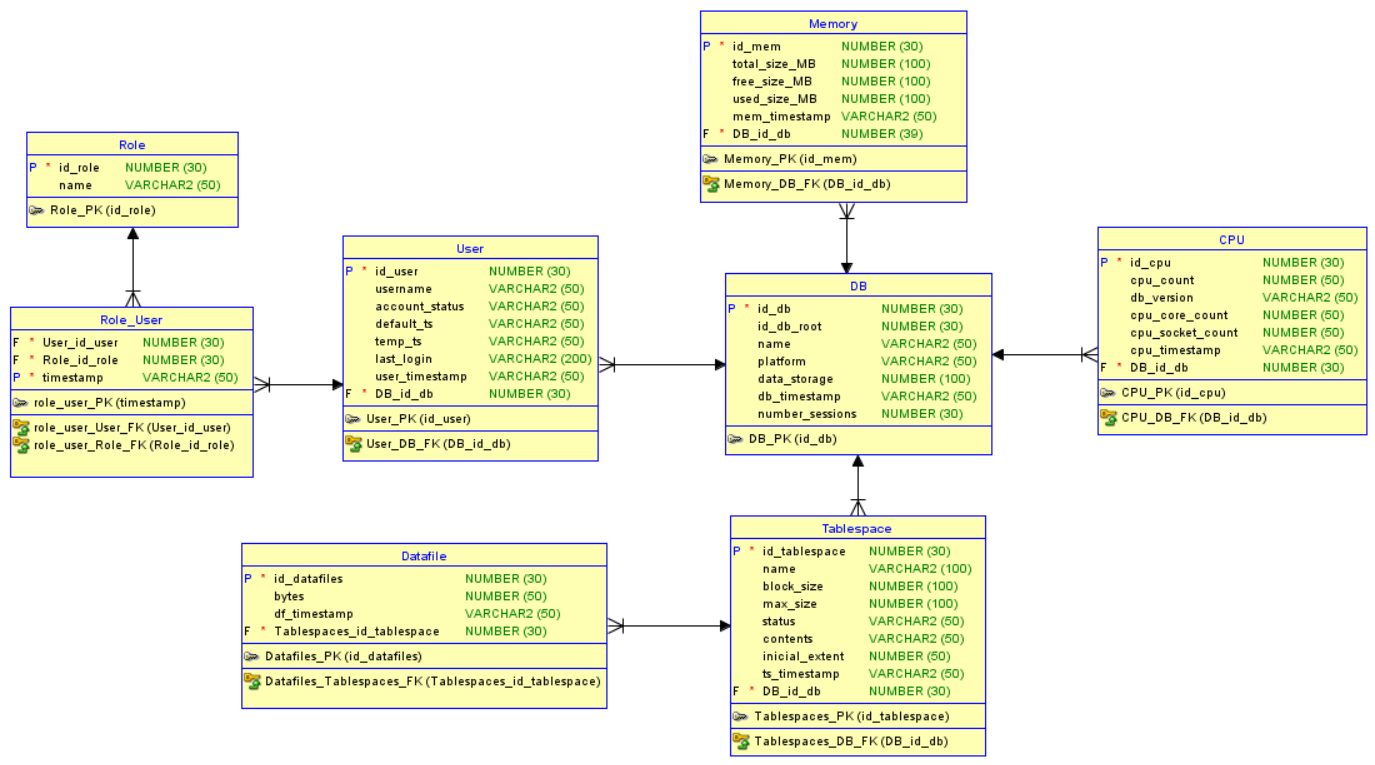
\includegraphics[scale=0.6]{modelo_logico.png}
\caption{Modelo Lógico}
\end{figure}

Como se pode verificar, considerou-se que uma base de dados é constituída por vários elementos de memória, \emph{cpu}, utilizadores e \emph{tablespaces}, ao passo que estes últimos pertencem a apenas uma base de dados. Uma \emph{tablespace} é composta por vários \emph{datafiles} e cada um destes está associado a apenas uma \emph{tablespace}. Já os utilizadores podem ter um conjunto de \emph{roles} e estes, por sua vez, podem ser empregados por utilizadores diferentes (N-N).


\subsection{Validação}
\hspace{3mm} 
De forma a validar o modelo de base de dados desenvolvido, começou-se por garantir a normalização desta. 

Com o objetivo de assegurar que este cumpra a \textbf{primeira forma normal}, foi necessário ter em atenção a relação N-N \textbf{(user-role)} no modelo lógico. Para lidar com este relacionamento, criou-se uma tabela intermediária que garantisse a atomicidade das colunas (atributos). 

Através da existência da chave primária \emph{\textbf{id}} em cada tabela, podemos garantir que todos os atributos dessa tabela estão dependentes desse mesmo \emph{id}, cumprindo assim a \textbf{segunda forma normal}. 

Por fim, visto que o nosso esquema se encontra na segunda forma normal e que nenhum atributo é dependente de um outro atributo dessa mesma tabela, exceto a chave primária, prova-se assim a \textbf{terceira forma normal} e demonstra-se que o modelo lógico se encontra normalizado.\\

Uma outra forma de testar/validar este esquema será executando interrogações relevantes ao projeto a desenvolver. Para tal foram desenvolvidas três \emph{queries} básicas que pretendem testar o modelo lógico e a sua capacidade de resposta:
\begin{itemize}
    \item Obter o número de \emph{bytes} alocados por uma determinada base de dados;
    \item Obter o número total de \emph{tablespaces} que estão a ser monitorizadas;
    \item Obter o nome do \emph{role} de um determinado utilizador;
\end{itemize}

\hspace{2mm} 

Um pequeno esboço dessas \emph{queries} comprova a validação do esquema desenvolvido:


\begin{itemize}
    \item \texttt{SELECT total\_size\_MB FROM Memory WHERE DB\_id\_db = X};
    \item \texttt{SELECT count(id\_tablespaces) FROM tablespaces};
    \item \texttt{SELECT name FROM role INNER JOIN role\_user on role.id\_role \\= role\_user.Role\_id\_role WHERE User\_id\_user = X };
\end{itemize}

Visto que é possível dar resposta a estas \emph{queries}, através do modelo lógico, podemos considerar que este é válido e pronto para ser implementado/ traduzido para o modelo físico. 

\subsection{Utilizador}
\label{users}
\hspace{3mm} 
De forma a ser possível obter a informação necessária para preencher a base de dados, será necessário aceder a diversas \emph{views}, para tal serão precisos \emph{users} que tenham acessos a estas. O \emph{user} que tipicamente tem esse acesso é o \emph{sys}, e visto que se pretende recolher não só informação da \emph{plugable DB} como também da \emph{root DB}, os \emph{sys} de ambas BDs serão necessários.

Por fim, um terceiro utilizador - \emph{grupo2} - foi criado, para gerar o modelo físico da base de dados que guardará as informações relevantes para o projeto.
A este utilizador foram associadas as \emph{tablespaces} \emph{TP\_AEBD e TP\_TEMP} e respetivos \emph{datafiles}, descritos mais à frente. Foi também atribuído o role de \textbf{DBA} e concedidas as permissões de criação de sessão (para se conectar à base de dados) e de criação de tabelas, para ser possível criar o modelo físico.


\begin{lstlisting}[ style = SQL ]
                    
-- USER grupo2
CREATE USER grupo2 IDENTIFIED BY pass  
DEFAULT TABLESPACE TP_AEBD
TEMPORARY TABLESPACE TP_TEMP
PASSWORD EXPIRE ;

ALTER USER grupo2 QUOTA UNLIMITED ON TP_AEBD;

-- GRANTS to grupo2
GRANT "DBA" TO grupo2 ;

GRANT CREATE SESSION TO grupo2 ;
GRANT CREATE TABLE TO grupo2 ;

-- TEST CONNECTION
connect grupo2/pass;

show user;  
                    
\end{lstlisting}


\subsubsection{Tablespaces \& Datafiles associados}
\hspace{3mm}

Foram criadas uma \emph{tablespace} permanente e uma temporária, denominadas \emph{TP\_AEBD e TP\_TEMP} respetivamente, para serem associadas ao utilizador \textbf{\emph{grupo2}}. A \emph{tablespace TP\_AEBD} irá ser responsável para guardar objetos de uma forma persistente durante as transações e sessões do utilizador. Esta contem o \emph{datafile TP\_AEBD\_01.dbf}. Já a \emph{TP\_TEMP} tem associado o \emph{tempfile TP\_TEMPORARY\_01.dbf} e irá armazenar objetos de uma forma temporária, com o objetivo de auxiliar em vários processamentos de \emph{queries} e outras operações na base de dados. 

\begin{lstlisting}[ style = SQL ]

-- TABLESPACE TP_AEBD
CREATE TABLESPACE TP_AEBD 
    DATAFILE 
        '\u01\app\oracle\oradata\orcl12\orcl\TP_AEBD_01.DBF' SIZE 104857600;

-- TABLESPACE TP_TEMP   
CREATE TEMPORARY TABLESPACE TP_TEMP 
    TEMPFILE 
        '\u01\app\oracle\oradata\orcl12\orcl\TP_TEMPORARY_01.DBF' SIZE 52428800 AUTOEXTEND ON NEXT 104857600 MAXSIZE 34359721984 
    EXTENT MANAGEMENT LOCAL UNIFORM SIZE 1048576;                    
                    
\end{lstlisting}

\subsection{Modelo Físico}
\hspace{3mm} 

Para a implementação física da base de dados, recorreu-se ao sistema de gestão de base de dados \textbf{\emph{Oracle SQL Developer}.} 

\subsubsection{Criação de tabelas}
\hspace{3mm}

Para efetuar a tradução do esquema lógica para a implementação física, o grupo estruturou as definições de cada uma das tabelas em linguagem de definição de dados (DDL), seguindo o desenho do modelo lógico realizado anteriormente, com o objetivo de criar as ditas tabelas.

As declarações \emph{CREATE e DROP}, criam e eliminam objetos que estão na base de dados, respetivamente, contidos no sistema de gestão de base de dados.

Em baixo, segue-se o \emph{script} de criação das tabelas da nossa base de dados "monitor" (tendo em atenção que as operações DROP estão em comentário, ficando sem efeito):

\begin{lstlisting}[ style = SQL ]
                    
-- TABLE DROPS
-- DROP TABLE Memory PURGE;
-- DROP TABLE CPU PURGE;
-- DROP TABLE Datafile PURGE;
-- DROP table UsersDB cascade constraints;
-- DROP TABLE Role cascade constraints;
-- DROP TABLE role_user cascade constraints;
-- DROP TABLE Tablespace PURGE;
-- DROP TABLE DB PURGE; 


-- DATABASE
CREATE TABLE db(
    id_db number(30) NOT NULL,
    id_db_root number(30) NOT NULL,
    name varchar(200) NOT NULL,
    platform varchar(20) NOT NULL,
    data_storage number(20) NOT NULL,
    number_sessions number(20) NOT NULL,
    db_timestamp varchar(50) NOT NULL,
    CONSTRAINT id_db PRIMARY KEY (id_db)
    );
    
-- MEMORY    
CREATE TABLE memory(
    id_mem          NUMBER(30) NOT NULL,
    total_size_mb   NUMBER(30),
    free_size_mb    NUMBER(30),
    used_size_mb    NUMBER(30),
    mem_timestamp   varchar(50),
    id_db_FK        NUMBER(30) NOT NULL,
    CONSTRAINT id_mem PRIMARY KEY (id_mem),
    CONSTRAINT id_db_memory
        FOREIGN KEY (id_db_FK)
        REFERENCES db(id_db)
    );
    
-- CPU
CREATE TABLE cpu(
    id_cpu number(30) NOT NULL,
    cpu_count number(20) NOT NULL,
    db_version varchar(70) NOT NULL,
    cpu_core_count number(20) NOT NULL,
    cpu_socket_count number(20) NOT NULL,
    cpu_timestamp varchar(50) NOT NULL,
    id_db_FK number(30) NOT NULL,
    CONSTRAINT id_cpu PRIMARY KEY (id_cpu),
    CONSTRAINT id_db_cpu
        FOREIGN KEY (id_db_FK)
        REFERENCES db(id_db)
    );

-- USER
CREATE TABLE usersDB(
    id_user number(30) NOT NULL,
    username varchar(70) NOT NULL,
    account_status varchar(70) NOT NULL,
    default_ts varchar(70) NOT NULL,
    temp_ts varchar(70) NOT NULL,
    last_login varchar(200) NOT NULL, 
    user_timestamp varchar(50) NOT NULL,
    id_db_FK number(30) NOT NULL,
    CONSTRAINT id_user PRIMARY KEY (id_user),
    CONSTRAINT id_db_users
        FOREIGN KEY (id_db_FK)
        REFERENCES db(id_db)
    );

-- ROLE
CREATE TABLE role(
    id_role number(30) NOT NULL,
    name varchar(70) NOT NULL,
    CONSTRAINT id_role PRIMARY KEY (id_role)
    );

-- ROLE AND USER
CREATE TABLE role_user(
    user_id_user   NUMBER(30) NOT NULL,
    role_id_role   NUMBER(30) NOT NULL,
    timestamp      VARCHAR2(50),
    CONSTRAINT role_user_user_fk 
        FOREIGN KEY ( user_id_user )
        REFERENCES usersdb ( id_user ),
    CONSTRAINT role_user_role_fk 
        FOREIGN KEY ( role_id_role )
        REFERENCES role ( id_role )
    );


-- TABLESPACE
CREATE TABLE tablespace(
    id_tablespace number(30) NOT NULL,
    name varchar(100) NOT NULL,
    block_size number(20) NOT NULL,
    max_size number(20) NOT NULL,
    status varchar(20) NOT NULL,
    contents varchar(30) NOT NULL,
    initial_extent number(20) NOT NULL,
    ts_timestamp varchar(50) NOT NULL,
    id_db_FK number(30) NOT NULL,
    CONSTRAINT id_tablespace PRIMARY KEY (id_tablespace),
    CONSTRAINT id_db_tablespace
        FOREIGN KEY (id_db_FK)
        REFERENCES db(id_db)
    );

-- DATAFILE
CREATE TABLE datafile(
    id_datafile number(30) NOT NULL,
    name varchar(150) NOT NULL,
    bytes number(20) NOT NULL,
    id_tablespace_FK numeric(20) NOT NULL,
    df_timestamp varchar(50) NOT NULL,
    CONSTRAINT id_datafile PRIMARY KEY (id_datafile),
    CONSTRAINT id_tablespace_datafile
        FOREIGN KEY (id_tablespace_FK)
        REFERENCES tablespace(id_tablespace)
    );
                    
\end{lstlisting}

\subsubsection{Sequences \& Triggers}
\hspace{3mm}

Para ter uma perspetiva da dimensão temporal, quanto à recolha de dados e estatísticas pelo monitor, e assim organizar um histórico da informação contida na PDB sob análise, foram colocados os atributos \emph{timestamp.} Além disso, cada instância de uma entidade (tabela) pode ser distinguida pelo seu \emph{id} único. Como o agente de recolha (monitor) estará constantemente a recolher informação da PDB, o grupo decidiu que os \textbf{ids únicos} de cada instância deveriam ser preenchidos \textbf{automaticamente}, pelo que cada id corresponde a uma determinada recolha num certo momento (identificado pelo \emph{timestamp}).

Visto que em Oracle SQL não é possível ter a opção de \emph{auto-increment} (em que os valores de \emph{ids} vão incrementando automaticamente), criou-se e utilizou-se \emph{sequences e triggers} para obter esse efeito. Desta forma, os \textbf{ids} de cada uma das entidades serão obtidos pelas sequências e vão incrementando antes de cada inserção, através dos \emph{triggers}.

Assim, uma dada sequência irá ser iniciada no valor 1. Posteriormente, antes de se inserir uma nova instância de uma dada entidade na base de dados, será ativado o respetivo \emph{trigger} para que o novo \emph{id} da instância a inserir possua o valor da sequência respetiva e, de seguida, o valor dessa sequência seja incrementado.

\begin{lstlisting}[ style = SQL ]
                    
-- SEQUENCE DROPS
-- DROP sequence db_seq;
-- DROP sequence memory_seq;
-- DROP sequence cpu_seq;
-- DROP sequence usersdb_seq;
-- DROP sequence role_seq;
-- DROP sequence tablespace_seq;
-- DROP sequence datafile_seq;

-- SEQUENCES
CREATE sequence db_seq start with 1 increment by 1 nomaxvalue;
CREATE sequence memory_seq start with 1 increment by 1 nomaxvalue;
CREATE sequence cpu_seq start with 1 increment by 1 nomaxvalue;
CREATE sequence usersdb_seq start with 1 increment by 1 nomaxvalue;
CREATE sequence role_seq start with 1 increment by 1 nomaxvalue;
CREATE sequence tablespace_seq start with 1 increment by 1 nomaxvalue;
CREATE sequence datafile_seq start with 1 increment by 1 nomaxvalue;


-- TRIGGERS
CREATE OR REPLACE TRIGGER db_trigger
BEFORE INSERT ON db
FOR EACH ROW
 WHEN (new.id_db IS NULL) 
BEGIN
  SELECT  db_seq.nextval
  INTO :new.id_db
  FROM dual;
END;
/

CREATE OR REPLACE TRIGGER memory_trigger
BEFORE INSERT ON memory
FOR EACH ROW
 WHEN (new.id_mem IS NULL) 
BEGIN
  SELECT  memory_seq.nextval
  INTO :new.id_mem
  FROM dual;
END;
/


CREATE OR REPLACE TRIGGER cpu_trigger
BEFORE INSERT ON cpu
FOR EACH ROW
 WHEN (new.id_cpu IS NULL) 
BEGIN
  SELECT  cpu_seq.nextval
  INTO :new.id_cpu
  FROM dual;
END;
/
        

CREATE OR REPLACE TRIGGER usersDB_trigger
BEFORE INSERT ON usersDB
FOR EACH ROW
 WHEN (new.id_user IS NULL) 
BEGIN
  SELECT  usersDB_seq.nextval
  INTO :new.id_user
  FROM dual;
END;
/


CREATE OR REPLACE TRIGGER role_trigger
BEFORE INSERT ON role
FOR EACH ROW
 WHEN (new.id_role IS NULL) 
BEGIN
  SELECT  role_seq.nextval
  INTO :new.id_role
  FROM dual;
END;
/  
        

CREATE OR REPLACE TRIGGER tablespace_trigger
BEFORE INSERT ON tablespace
FOR EACH ROW
 WHEN (new.id_tablespace IS NULL) 
BEGIN
  SELECT  tablespace_seq.nextval
  INTO :new.id_tablespace
  FROM dual;
END;
/  
        

CREATE OR REPLACE TRIGGER datafile_trigger
BEFORE INSERT ON datafile
FOR EACH ROW
 WHEN (new.id_datafile IS NULL) 
BEGIN
  SELECT  datafile_seq.nextval
  INTO :new.id_datafile
  FROM dual;
END;
/         

\end{lstlisting}

\section{Ligação à Base de Dados - Java API}
\label{ligacaoBD}
\hspace{3mm} 

Para interagir com o servidor Oracle, foi desenvolvida uma aplicação com a linguagem de programação \emph{Java} - \textbf{o agente de recolha de informação}.

Esta serviu para realizar as conexões ao servidor da base de dados, enviar os comandos SQL a serem executados e recolher os resultados dos mesmos. A ferramenta utilizada para ser possível comunicar com o sistema da base de dados e realizar estas operações foi \emph{\textbf{JDBC} (Java Database Connectivity)}.

O \emph{JDBC} permite consultar e atualizar dados contidos na base de dados, bem como obter resultados de várias \emph{queries} que o utilizador pretenda executar. Isto é bastante útil para explorar as relações existentes entres os diversos dados que estão na base de dados e obter informações destes, como o seu nome e tipo (\emph{metadados}).

Os passos básicos para comunicar com a base de dados, através desta API, podem ser resumidos da seguinte forma:

\begin{enumerate}
    \item Formar uma conexão com a base de dados;
    
    \item Criar um objeto "\emph{statement}";
    
    \item Utilizar o objeto "\emph{statement}"\ para enviar as \emph{queries} que se pretende realizar e recolher os resultados destas;
    
    \item Utilizar mecanismos de excepção para lidar com potenciais erros;
\end{enumerate}

No agente monitor, a classe \emph{\textbf{BDConnection}} é a responsável por criar e gerir as sessões e conexões às várias bases de dados Oracle, segundo os utilizadores \emph{sys} e \emph{grupo2}.

A API de \emph{JDBC} foi implementada através da \emph{OracleDriver}, que fornece classes para instalar as interfaces de \emph{JDBC} e assim permitir processar os seus pedidos e retornar os resultados à aplicação em \emph{Java} (agente).

Foram também configuradas as conexões às bases de dados \emph{CDB e PDB}, pelos os users \emph{sys e grupo2}. Conectamos a aplicação à CDB, através do \emph{driver}, fazendo uma ligação ao endereço correspondente: \emph{localhost:1521:orcl12c}. Este endereço justifica-se pelo facto do servidor da base de dados \emph{Oracle} ser executado numa máquina virtual na própria máquina do grupo, na porta 1521, em que \emph{orcl12} é a designação da CDB Oracle. Já para se conectar à PDB, efetua-se uma ligação ao endereço \emph{localhost:1521/orcl}, já que \emph{orcl} é a sua designação.

As funções da classe \emph{BDConnection} são detalhadas na secção seguinte.

\begin{lstlisting}[ style = JAVA ]
public class BDConnection
    
    // Driver
    public static final String DB_DRIVER = "oracle.jdbc.driver.OracleDriver";
    
    // Connection to the CDB
    public static final String DB_CONNECTION_ROOT = "jdbc:oracle:thin:@localhost:1521:orcl12c";
    
    // Connection to the PDB
    public static final String DB_CONNECTION_PLUG = "jdbc:oracle:thin:@localhost:1521/orcl";
    
    // User sys
    public static final String DB_USER = "sys as sysdba";
    public static final String DB_PASSWORD = "oracle";
    
    // User grupo
    public static final String DB_USER_GROUP = "grupo2";

\end{lstlisting}


\section{Agente de Recolha de Informação}
\hspace{3mm} 

Visto os métodos utilizados para efetuar ligações às bases de dados, seguem-se as descrições detalhadas das classes da aplicação desenvolvida em Java. Como dito anteriormente, esta tem o objetivo de monitorizar a PDB \emph{orcl} e guardar a informação obtida nas base de dados "monitor", desenvolvida pelo grupo. 

O Agente de Recolha de Informação apresenta as seguintes classes:
\begin{itemize}
    \item \textbf{BDConnection};
    \item \textbf{Selects};
    \item \textbf{Inserts};
    \item \textbf{Monitor};
    \item \textbf{Main}.
\end{itemize}

\subsection{Classes}

\subsubsection{BDConnection}
\label{bdconnection}
\hspace{3mm} 

A classe \emph{BDConnection} estabelece a ligação às Bases de Dados através dos diferentes utilizadores.  Utiliza o utilizador \emph{sys}, tanto para a \emph{pluggable} DB (PBD) como para a \emph{Root} DB (CDB), visto que será necessário aceder a ambas, por forma a obter informação especifica. 
É também  estabelecida a conexão a um utilizador pertencente à \emph{pluggable} DB, \emph{grupo2}, possuindo acesso à Base de Dados "monitor",  que irá guardar toda a informação recolhida.
As técnicas para formar esta ligação estão descritas na secção \ref{ligacaoBD} - \textbf{Ligação à Base de Dados}.\\

A função \emph{getBDConnection} recebe como parâmetros um objeto conexão, um \emph{username} e uma \emph{password}, para estabelecer uma ligação a uma determinada base de dados, segundo as credenciais de um utilizador. As funções getBDConnection\_root(), getBDConnection\_plug() e getBDConnection\_group formam conexões com os utilizadores \emph{sys.cdb, sys.orcl e grupo2}, respetivamente, em que a primeira relaciona-se com a CDB (root) e as restantes com a \emph{pluggable} DB.

\begin{lstlisting}[ style = JAVA ]

// Conexao generica
public static Connection getBDConnection(String conn, String user, String pw);

// Conexao sys.cdb
getBDConnection_root(): return getBDConnection(DB_CONNECTION_ROOT, DB_USER, DB_PASSWORD);
// Conexao sys.orcl
getBDConnection_plug(): return getBDConnection(DB_CONNECTION_PLUG, DB_USER, DB_PASSWORD);
// Conexao grupo2.orcl
getBDConnection_group(): return getBDConnection(DB_CONNECTION_PLUG, DB_USER_GROUP, DB_PASSWORD);

\end{lstlisting}

\subsubsection{Selects}
\label{selects}
\hspace{3mm} 

Já a classe \emph{Selects} é responsável pela recolha de informação relativamente aos parâmetros de avaliação da \emph{performance} da Base de Dados \emph{Oracle}, definidos pelo grupo. Sendo assim, esta classe verifica qual a informação a obter, liga-se ao utilizador \emph{sys} da \emph{root} ou da \emph{pluggable} DB de acordo com o parâmetro desejado e, através de um \emph{SELECT} simples, seleciona/recolhe esses dados.

Como dito anteriormente, por forma a preencher as tabelas da nossa base de dados "monitor", teremos de ter em conta as \emph{views} disponíveis (já existentes) da base de dados \emph{pluggable} que queremos monitorizar, de modo a coletar informação, dados e estatísticas desta.
Eis a relação entre as tabelas e as \emph{views}, para inserção de dados e preenchimento da base de dados "monitor":\\

\textbf{\large DB}\\

Com o objetivo de preencher a tabela DB, responsável por armazenar dados relativos à base de dados \emph{pluggable}, extraímos informação da \emph{view} \textbf{\emph{V\$DATABASE}} disponível na \emph{pluggable} DB, através do utilizador \emph{sys}.

Os parâmetros selecionados para serem armazenados são os seguintes: \textbf{DBID}, \textbf{NAME} e \textbf{PLATAFORM\_NAME}.\\

\begin{lstlisting}[ style = JAVA ]
public static ResultSet selectDB() 
            PreparedStatement ps = c_plug.prepareStatement("SELECT DBID, NAME, PLATFORM_NAME FROM V$DATABASE");

\end{lstlisting}

Tendo em conta o modelo lógico, é possível identificar o parâmetro \emph{number\_sessions}, que é obtido através de um contagem no número de sessões guardadas na \emph{view} \emph{V\$SESSION}, que se encontra na \emph{root} DB (CDB).


\begin{lstlisting}[ style = JAVA ]
public static String selectNrSessions() 
            ps = c_root.prepareStatement("SELECT COUNT(*) FROM V_$SESSION");

\end{lstlisting}

\textbf{\large Memory}\\

Para realizar o preenchimento da tabela \emph{memory}, que representam os custos relacionados com o uso de memória da \emph{database}, foi utilizada a \emph{view} \emph{V\$SGA} para obter a memória total disponível e \emph{V\$SGASTAT} para obter a quantidade de memória livre disponível à \emph{DataBase}. Ambas as \emph{views} encontram-se na \emph{root} DB (CDB) e são acedidas através do utilizador \emph{sys}. 
Um valor importante que é guardado na base de dados é a memória a ser utilizada no momento de recolha. Para tal, quando se insere os dados na base de dados, esse valor é calculado, através da subtração do espaço total da memória existente e o espaço disponível.

\begin{lstlisting}[ style = JAVA ]
public static ResultSet selectMemory_totalSizeMB() 
            ps = c_root.prepareStatement("SELECT round(SUM(value)/1024/1024) FROM V_$SGA");

\end{lstlisting}

\begin{lstlisting}[ style = JAVA ]
public static ResultSet selectMemory_freeSizeMB() 
            ps = c_root.prepareStatement("SELECT round(SUM(bytes/1024/1024)) FROM V_$SGASTAT Where Name Like '%free memory%'");

\end{lstlisting}

\textbf{\large CPU}\\

De forma a armazenar os valores relacionados com o custo de \emph{CPU} da DB, é necessário primeiro especificar o identificador da base de dados a monitorizar. No nosso caso, visto que se trata da \emph{orcl}, foi possível perceber que o id dessa base de dados é \textbf{776972821}. Tendo isto em conta, foi usada a \emph{view} \emph{DBA\_CPU\_USAGE\_STATISTICS} da \emph{root} com o utilizador \emph{sys} desta.

\begin{lstlisting}[ style = JAVA ]
public static ResultSet selectCPU() 
            ps = c_root.prepareStatement("SELECT *  FROM DBA_CPU_USAGE_STATISTICS where dbid = 776972821");

\end{lstlisting}


\textbf{\large UsersDB}\\

Com o objetivo de armazenar os dados referentes aos utilizadores da DB foi necessário recorrer à \emph{view} presente na \emph{pluggable} DB, \emph{DBA\_USERS}. É também importante referir que quando a data do \emph{last\_login} não está definida, esta é substituída por um \emph{'undefined'}.

\begin{lstlisting}[ style = JAVA ]
public static ResultSet selectUser() 
            ps = c_plug.prepareStatement("SELECT USERNAME, ACCOUNT_STATUS, DEFAULT_TABLESPACE, TEMPORARY_TABLESPACE, NVL(TO_CHAR(LAST_LOGIN),'undefined') FROM DBA_USERS");

\end{lstlisting}

\textbf{\large Role}\\

Para ser possível ter acesso à informação referente aos \emph{roles} que a base de dados a monitorizar oferece aos seus utilizadores, considerou-se necessário guardar essa informação também. Para tal, é utilizada a \emph{view} \emph{DBA\_ROLES} presente na \emph{pluggable} DB, através do seu utilizador \emph{sys}.

\begin{lstlisting}[ style = JAVA ]
public static ResultSet selectRole() 
            ps = c_plug.prepareStatement("SELECT ROLE_ID, ROLE FROM DBA_ROLES");

\end{lstlisting}

\textbf{\large Datafile}\\

De forma a guardar os dados relativos aos \emph{Datafiles} pertencentes a um \emph{tablespace} existentes na base de dados a monitorizar, são utilizadas as \emph{views} \emph{DBA\_TEMP\_FILES} e \emph{DBA\_DATA\_FILES}, para os \emph{datafiles} temporários e permanentes, respetivamente. Para isso utiliza-se o utilizador \emph{sys.orcl}.

\begin{lstlisting}[ style = JAVA ]
public static ResultSet selectDatafile() 
            ps = c_plug.prepareStatement("SELECT FILE_NAME, BYTES, TABLESPACE_NAME  FROM DBA_DATA_FILES UNION SELECT FILE_NAME, BYTES, TABLESPACE_NAME  FROM DBA_TEMP_FILES");

\end{lstlisting}

\textbf{\large Tablespace}\\

Por fim, para guardar a informação referente aos \emph{Tablespaces} é necessário aceder à \emph{view} \emph{DBA\_TABLESPACES}, que pertence à \emph{pluggable} DB, através do utilizador \emph{sys} correspondente.

\begin{lstlisting}[ style = JAVA ]
public static ResultSet selectTablespace() 
            ps = c_plug.prepareStatement("SELECT TABLESPACE_NAME, BLOCK_SIZE,  MAX_SIZE, STATUS, CONTENTS, INITIAL_EXTENT  FROM DBA_TABLESPACES");
\end{lstlisting}

\newpage

\subsubsection{Inserts}
\hspace{3mm} 

Por sua vez, a classe \emph{Inserts} gere a inserção de dados na Base de Dados "monitor". Para tal, utiliza a conexão referente ao utilizador \emph{\textbf{Grupo2}}, previamente criada, e executa um \emph{INSERT} simples, a partir dos dados obtidos através das \emph{views} na classe \emph{Selects}. É assim realizado o armazenamento dos dados sobre a \emph{performance} da Base de Dados \emph{pluggable} em questão. 

A \emph{query} de inserção é executada através de um \emph{Statement}, em que os valores a inserir são preenchidos com os dados respetivos extraídos do \emph{ResultSet}, recebido como argumento, resultante das operações \emph{Select} executadas anteriormente.

Tendo em conta a existência habitual de chaves estrangeiras na base de dados a preencher, foi importante utilizar uma abordagem do interior para o exterior, isto é, preencher primeiramente as tabelas que não possuem chaves estrangeiras entre elas a \emph{DB}, pois todas as tabelas que a rodeiam dependem do identificador desta, e depois as tabelas que possuem essas chaves estrangeiras. A base de dados que é utilizada para monitorizar o sistema é criada e gerida pelo utilizador \emph{grupo2}.\\


\textbf{\large DB}\\

Com o objetivo de inserir os dados na tabela DB, utiliza-se um \emph{Insert} baseado nos resultados do \emph{Select} da base de dados, obtidos anteriormente:

\begin{lstlisting}[ style = JAVA ]
public static void initDB() 
            s =  "insert into db (id_db_root, name, platform, data_storage, db_timestamp, number_sessions) values (?,?,?,(Select sum(bytes) from DBA_DATA_FILES) ,?,?)";
\end{lstlisting}


\textbf{\large Memory}\\

De forma a inserir os dados na tabela referente à memória utiliza-se um \emph{Insert} baseado nos resultados do \emph{Select} da memória obtidos anteriormente:

\begin{lstlisting}[ style = JAVA ]
public static void insertMemory() 
            s =  "insert into memory (total_size_mb, free_size_mb, used_size_mb, mem_timestamp, id_db_FK) values (?,?,?-?,?,db_seq.CURRVAL)";
\end{lstlisting}

\textbf{\large CPU}\\

De forma a inserir os dados na tabela referentes ao custo de CPU utiliza-se um \emph{Insert} baseado nos resultados do \emph{Select} do CPU obtidos anteriormente:

\begin{lstlisting}[ style = JAVA ]
public static void insertCPU() 
            s = "insert into cpu (cpu_count, db_version, cpu_core_count, cpu_socket_count, cpu_timestamp, id_db_FK) values (?,?,?,?,?,db_seq.CURRVAL)";

\end{lstlisting}

\textbf{\large UsersDB}\\

De forma a inserir os dados na tabela referentes aos \emph{users} existentes na DB utiliza-se um \emph{Insert} baseado nos resultados do \emph{Select} dos utilizadores obtidos anteriormente:

\begin{lstlisting}[ style = JAVA ]
public static void insertUsers() 
            s = "insert into usersDB (username, account_status, default_ts, temp_ts, last_login, user_timestamp, id_db_FK) values (?,?,?,?,?,?,db_seq.CURRVAL)";


\end{lstlisting}

\newpage

\textbf{\large Role}\\

De forma a inserir os dados na tabela referentes aos \emph{roles} existentes na DB utiliza-se um \emph{Insert} baseado nos resultados do \emph{Select} dos \emph{roles} obtidos anteriormente:

\begin{lstlisting}[ style = JAVA ]
public static void insertRole() 
            s = "insert into role (id_role, name) values (?,?)";


\end{lstlisting}

\textbf{\large Datafile}\\

De forma a inserir os dados na tabela referentes aos \emph{datafiles} pertencentes ao respetivo \emph{tablespace} na DB utiliza-se um \emph{Insert} baseado nos resultados do \emph{Select} dos \emph{datafiles} obtidos anteriormente:

\begin{lstlisting}[ style = JAVA ]
public static void insertDatafile() 
            s = "insert into datafile (name, bytes, df_timestamp, id_tablespace_FK) values (?,?,?,(SELECT id_tablespace from TABLESPACE where name = ? and ts_timestamp = ?))";


\end{lstlisting}

\textbf{\large Tablespace}\\

De forma a inserir os dados na tabela referentes aos \emph{tablespaces} existentes na DB utiliza-se um \emph{Insert} baseado nos resultados do \emph{Select} dos \emph{tablespaces} obtidos anteriormente:

\begin{lstlisting}[ style = JAVA ]
public static void insertTablespace() 
            s = "insert into tablespace (name, block_size, max_size, status, contents, initial_extent, ts_timestamp, id_db_FK) values (?,?,?,?,?,?,?,db_seq.CURRVAL)";

\end{lstlisting}

\subsubsection{Monitor}
\hspace{3mm} 

A classe Monitor tem como principal função conjungar os processos de recolha e armazenamento da informação pretendida. 

Inicialmente, com a execução do monitor, são realizados dois \emph{selects} necessários para o preenchimento da tabela DB (da base de dados "monitor") devido a esta ser completamente independente de todas as outras.  

Após isto, a base de dados responsável pelo armazenamento dos dados é inicializada e pronta para receber toda a informação pretendida.

O processo de recolha e de inserção da informação, das \emph{views} para a base de dados, é feita diretamente, isto é, sem qualquer tipo de armazenamento temporário mas sempre respeitando a dependência de cada tabela.

No final de cada ciclo de recolha é sempre tido em atenção a necessidade de terminar as conexões com a Base de Dados \emph{Oracle}.

\begin{lstlisting}[ style = JAVA ]
public static void start(){
        Selects sl = new Selects();                                  
        ResultSet rs = sl.selectDB();
        // Number of sessions
        String nr_sessions = sl.selectNrSessions();
        // Init DB
        Inserts in = new Inserts(sl);
        in.initDB(rs, nr_sessions);
\end{lstlisting}

\subsubsection{Main}
\hspace{3mm} 

Esta classe é responsável pelo início de todo o processo de recolha e armazenamento de dados, por parte do monitor. A recolha é feita em intervalos de 15 segundos para que seja possível observar a evolução da carga na performance da \emph{pluggable} DB e projetar um histórico de estatísticas com os principais parâmetros de avaliação do desempenho.\\

\begin{lstlisting}[ style = JAVA ]
public static void main(String[] args) throws SQLException  {
        while (true) {
            // Start
            Monitor.start();
            try {
                sleep(15000);
            }
\end{lstlisting}


\subsection{Tabela \emph{Source - Target} : Resumo}
\hspace{3mm} 

Esta tabela resume a relação entre os dados recolhidos na base de dados \emph{pluggable} (\textbf{origem}) e o preenchimento das estatísticas na base de dados monitor (\textbf{destino}).

\begin{table}[h!]
\resizebox{\textwidth}{!}{%
\begin{tabular}{|c|c|c|c|c|c|}
\hline
\multicolumn{3}{|c|}{{\ul \textbf{Origem}}} & \multicolumn{3}{c|}{{\ul \textbf{Destino}}} \\ \hline
\textbf{Base de Dados} & \textbf{Tabela} & \textbf{Atributo} & \textbf{Base de Dados} & \textbf{Tabela} & \textbf{Atributo} \\ \hline
PDB orcl & \textit{V\$DATABASE} & DBID & Monitor & \textit{DB} & id\_db\_root \\ \hline
PDB orcl & \textit{V\$DATABASE} & NAME & Monitor & \textit{DB} & name \\ \hline
PDB orcl & \textit{V\$DATABASE} & PLATFORM\_NAME & Monitor & \textit{DB} & platform \\ \hline
CDB root & \textit{V\_\$SESSION} & count(*) & Monitor & \textit{DB} & nr\_sessions \\ \hline
CDB root & DBA\_CPU\_USAGE\_STATISTICS & CPU\_COUNT & Monitor & \textit{CPU} & cpu\_count \\ \hline
CDB root & \textit{DBA\_CPU\_USAGE\_STATISTICS} & DB\_VERSION & Monitor & \textit{CPU} & db\_version \\ \hline
CDB root & \textit{DBA\_CPU\_USAGE\_STATISTICS} & CPU\_CORE\_COUNT & Monitor & \textit{CPU} & cpu\_core\_count \\ \hline
CDB root & \textit{DBA\_CPU\_USAGE\_STATISTICS} & CPU\_SOCKET\_COUNT & Monitor & \textit{CPU} & cpu\_socket\_count \\ \hline
CDB root & V\_\$SGA & VALUE & Monitor & \textit{MEMORY} & total\_size\_mb \\ \hline
CDB root & \textit{V\_\$SGASTAT} & BYTES & Monitor & \textit{MEMORY} & free\_size\_mb \\ \hline
PDB orcl & \textit{DBA\_TABLESPACES} & TABLESPACE\_NAME & Monitor & \textit{TABLESPACE} & name \\ \hline
PDB orcl & \textit{DBA\_TABLESPACES} & BLOCK\_SIZE & Monitor & \textit{TABLESPACE} & block\_size \\ \hline
PDB orcl & \textit{DBA\_TABLESPACES} & MAX\_SIZE & Monitor & \textit{TABLESPACE} & max\_size \\ \hline
PDB orcl & \textit{DBA\_TABLESPACES} & STATUS & Monitor & \textit{TABLESPACE} & status \\ \hline
PDB orcl & \textit{DBA\_TABLESPACES} & CONTENT & Monitor & \textit{TABLESPACE} & content \\ \hline
PDB orcl & \textit{DBA\_TABLESPACES} & INITIAL\_EXTENT & Monitor & \textit{TABLESPACE} & initial\_extend \\ \hline
PDB orcl & \textit{DBA\_TEMP\_FILE} & FILE\_NAME & Monitor & \textit{DATAFILE} & name \\ \hline
PDB orcl & \textit{DBA\_TEMP\_FILE} & BYTES & Monitor & \textit{DATAFILE} & bytes \\ \hline
PDB orcl & \textit{DBA\_ROLES} & ROLE\_ID & Monitor & \textit{ROLE} & id\_role \\ \hline
PDB orcl & \textit{DBA\_ROLES} & ROLE & Monitor & \textit{ROLE} & name \\ \hline
PDB orcl & \textit{DBA\_USERS} & USERNAME & Monitor & \textit{USER} & username \\ \hline
PDB orcl & \textit{DBA\_USERS} & ACCOUNT\_STATUS & Monitor & \textit{USER} & account\_status \\ \hline
PDB orcl & \textit{DBA\_USERS} & DEFAULT\_TABLESPACE & Monitor & \textit{USER} & default\_ts \\ \hline
PDB orcl & \textit{DBA\_USERS} & TEMPORARY\_TABLESPACE & Monitor & \textit{USER} & temp\_ts \\ \hline
PDB orcl & \textit{DBA\_USERS} & LAST\_LOGIN & Monitor & \textit{USER} & last\_login \\ \hline
\end{tabular}%
}
\end{table}

\newpage

\section{API REST}
\hspace{3mm} 

Os \emph{\textbf{Oracle REST Data Services (ORDS)}} permitem desenvolver interfaces \emph{REST} para Bases de Dados \emph{Oracle} relacionais. Foi através destes serviços, incorporados na aplicação \emph{SQL Developer}, que nos era fornecida a opção de inicialização de um serviço REST, pelo que se decidiu utilizar esta alternativa, de modo a facilitar e agilizar o processo.

\subsubsection{Ativação dos serviços REST para a BD}
\hspace{3mm} 

Em primeiro lugar, houve a necessidade de ativar os  \emph{\textbf{REST services}} para a ligação do nosso utilizador à Base de Dados -  \emph{\textbf{grupo2}}. Para isso, bastou ir à opção "REST Services"\ de \emph{\textbf{grupo2.orcl}}, onde ativamos os serviços REST em "\emph{Enable REST Services...}", visível na imagem abaixo:

\begin{figure}[H]
\centering
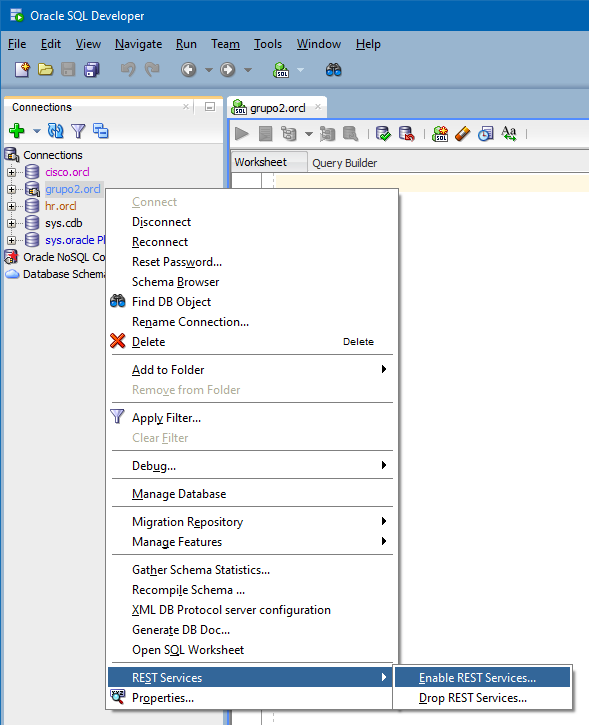
\includegraphics[scale=0.55]{REST/rest_grupo2_1.png}
\caption{Ativação dos serviços REST em grupo2.orcl}
\end{figure}

De seguida é nos apresentado o \emph{wizard} de configuração.
Na primeira janela \textbf{(figura 11)} marcamos a caixa \emph{"Enable schema"} e definimos o \emph{"Schema alias"} como \textbf{grupo2}. Este nome será necessário mais tarde nos pedidos \emph{web}. Se fosse pretendido uma maior segurança, seria possível mudar o \emph{alias} para algo diferente do nome original, bem como marcar a última caixa para ativar autenticação nos pedidos. No entanto, esta situação não foi considerada relevante para este trabalho.

\begin{figure}[H]
\centering
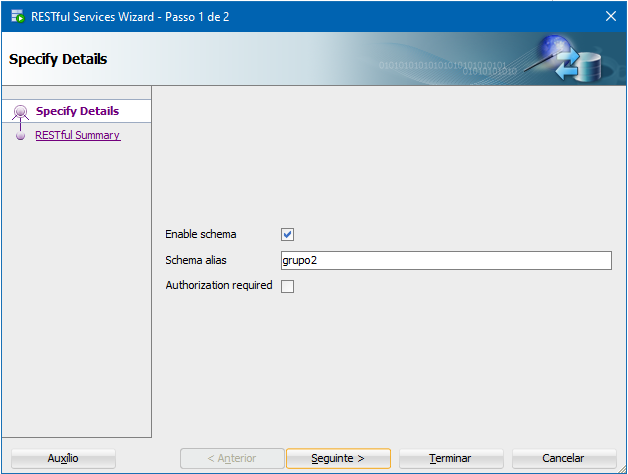
\includegraphics[scale=0.6]{REST/rest_grupo2_2.png}
\caption{Ativação dos serviços REST - Wizard}
\end{figure}

Nesta segunda janela, permite a confirmação das opções selecionadas préviamente e finaliza-se a configuração:

\begin{figure}[H]
\centering
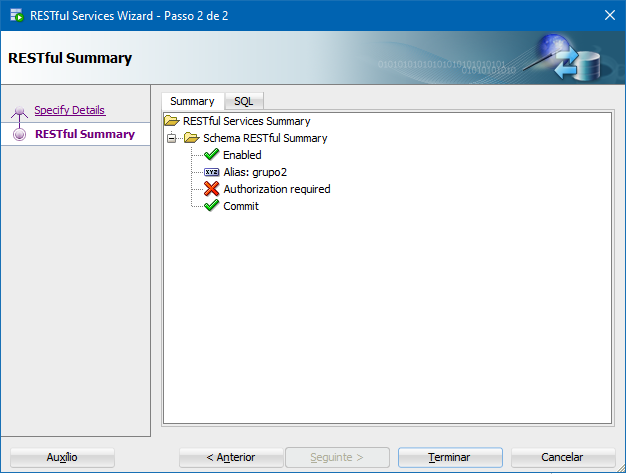
\includegraphics[scale=0.6]{REST/rest_grupo2_3.png}
\caption{Ativação dos serviços REST - Wizard}
\end{figure}

\subsubsection{Ativação das tabelas}
\hspace{3mm} 

Depois de ativar o \emph{REST service} na nossa ligação entre utilizador e BD -- \emph{\textbf{grupo2.orcl}}  --  falta ainda ativá-lo para todas as tabelas que pretendemos ter acesso \emph{via REST}, ou seja, todas as tabelas da nossa BD "monitor".
Segue-se um exemplo para a tabela CPU. O processo é o mesmo, nas opções da tabela selecionamos \emph{"Enable REST Services..."}, de forma a abrir o \emph{wizard}, como na imagem abaixo.

\begin{figure}[H]
\centering
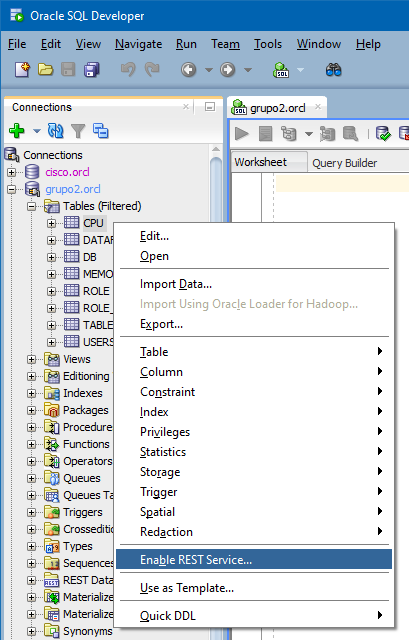
\includegraphics[scale=0.6]{REST/rest_tabela_1.png}
\caption{Ativação dos serviços REST na tabela CPU}
\end{figure}

Já no \emph{wizard} o processo é exatamente igual ao de ativação para a BD, apenas sendo necessário referir que todas as tabelas mantiveram um \emph{alias} igual ao nome da tabela, com exceção da tabela \textbf{USERSDB} que foi nomeado de \textbf{user} e da tabela  \emph{\textbf{ROLE\_USER}} que não foi ativada.\\

\subsubsection{API}
\hspace{3mm} 

Visto que a interface REST foi criada automaticamente pelos \emph{ORDS}, a API a utilizar foi a gerada consequentemente. Esta, por sua vez, mostrou-se muito prática e simples de aplicar.

Para obter um certo dado, executa-se um pedido \emph{GET} que, por sua vez, retorna um \textbf{JSON} com a informação pretendida.
Os pedidos seguem a seguinte fórmula:\\

$\bullet$ \texttt{http://localhost:8080/ords/\{\textbf{\emph{alias} da DB}\}/\{\textbf{\emph{alias} da tabela}\}/}\\

Na prática, basta substituir apenas os \textbf{"\emph{alias da DB"}} e \textbf{"\emph{alias da tabela}"}, pelos nomes correspondentes das tabelas que pretendemos aceder.

Segue-se, a título de exemplo, um pedido à PDB na tabela DB, com o utilizador \emph{grupo2}:

\begin{figure}[H]
\centering
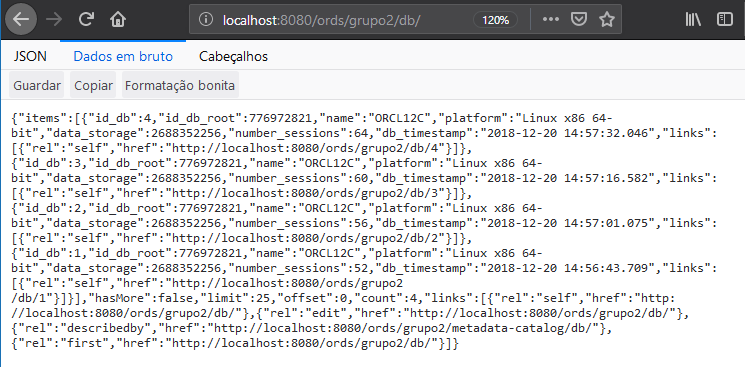
\includegraphics[scale=0.70]{REST/api_1.png}
\caption{Exemplo de um pedido GET a \textbf{grupo2:db}}
\end{figure}

É também possível efetuar GETs com maior precisão, adicionando condições à \emph{query}.
De seguida, apresenta-se a imagem de um exemplo onde utilizamos o pedido anterior como base, mas onde pretendemos apenas a entrada com \textbf{\emph{id\_db}} igual a 1.

\begin{figure}[H]
\centering
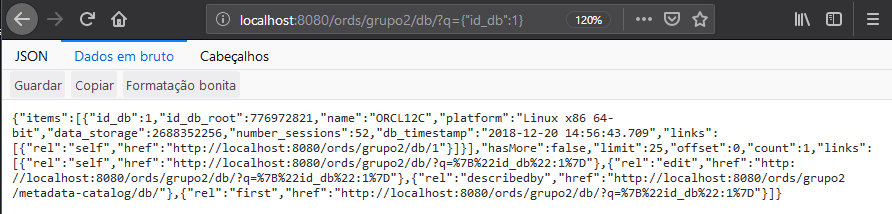
\includegraphics[scale=0.6]{REST/api_2.png}
\caption{Exemplo de um pedido GET ao grupo2:db}
\end{figure}

A API gerada permite também realizar pedidos de \emph{POST, PUT, DELETE}, entre outros, contudo estes não se mostraram necessários para o nosso trabalho.


\section{Interface Web}
\hspace{3mm} 

Numa última fase, o grupo desenvolveu uma interface \emph{web}, de modo a permitir ao utilizador uma visualização mais agradável e intuitiva sobre os dados do desempenho da base de dados \emph{pluggable}.

Isto foi possível ao interpretar o código JSON, gerado pelo serviço REST e que contem essa informação, e combiná-los com HTML, formando assim páginas \emph{web} onde se apresentassem os dados em forma de tabelas e gráficos.

Na interface \emph{web}, preparamos uma \emph{Homepage} com informações gerais sobre o projeto e o grupo, e separadamente criou-se uma página individual para cada tabela/entidade que pretendíamos visualizar, da base de dados "monitor".

\newpage

\subsection{Screenshots}
\hspace{3mm} 

Nesta secção é possível visualizar alguns \emph{screenshots} dos resultados finais da interface \emph{web}, em que cada imagem é seguida da sua respetiva legenda, contendo uma pequena descrição sobre a página \emph{web} que representa (as imagens monstram apenas uma parte da interface). Para testar e confirmar que eram recolhidos dados fidedignos da base de dados \emph{pluggable}, utilizou-se a ferramenta \emph{\textbf{Swingbench}} para gerar carga sob esta base de dados e assim obter flutuações nos valores dos dados recolhidos e registar as variações nos resultados, ficando visualmente mais perceptível a verificação da informação obtida.

\begin{figure}[H]
\centering
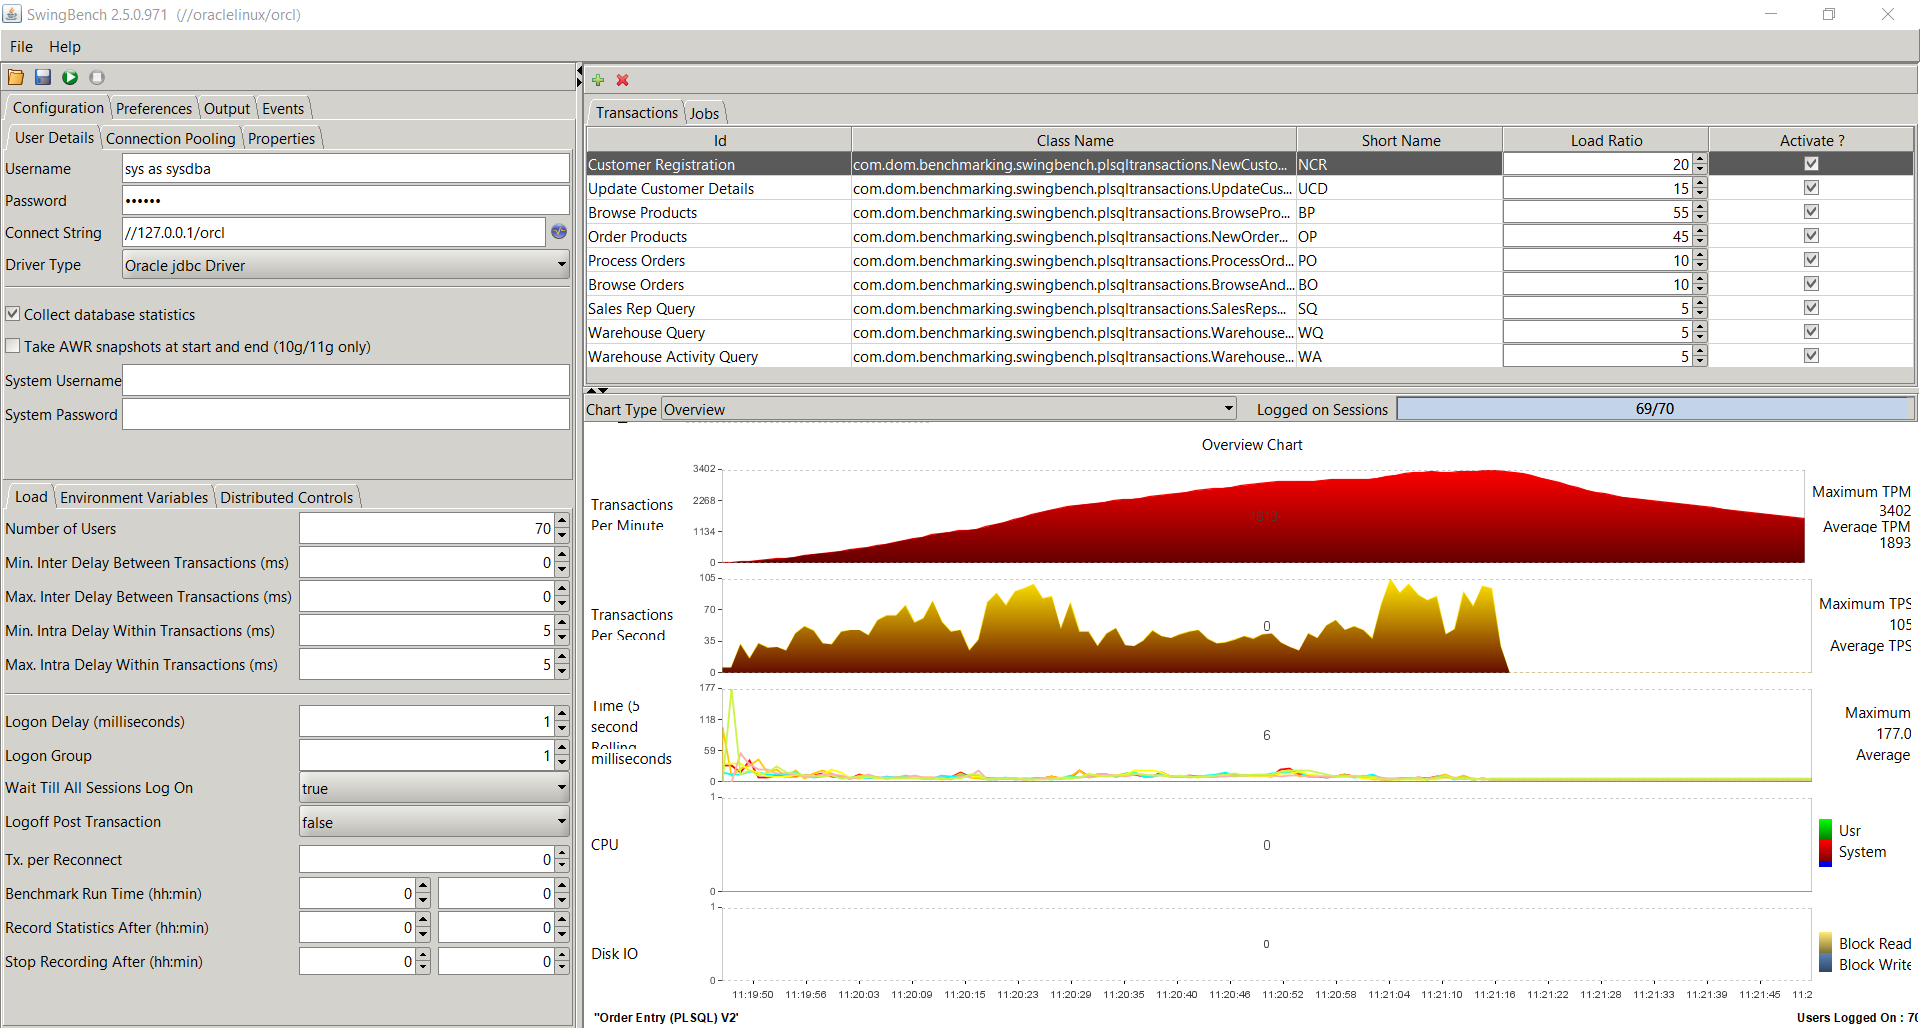
\includegraphics[scale=0.4]{html/swing.png}
\caption{Para permitir a ferramenta \emph{swingbench} de injetar carga na base de dados, indicamos o endereço desta (127.0.0.1/orcl) e utilizamos as credenciais do utilizador \emph{sys} para autorização. Utilizaram-se cerca de 70 utilizadores, cujas características das transações efetuadas encontram-se expostas no \emph{screenshot}, assim como a monitorização das operações realizadas.}
\end{figure}

\begin{figure}[H]
\centering
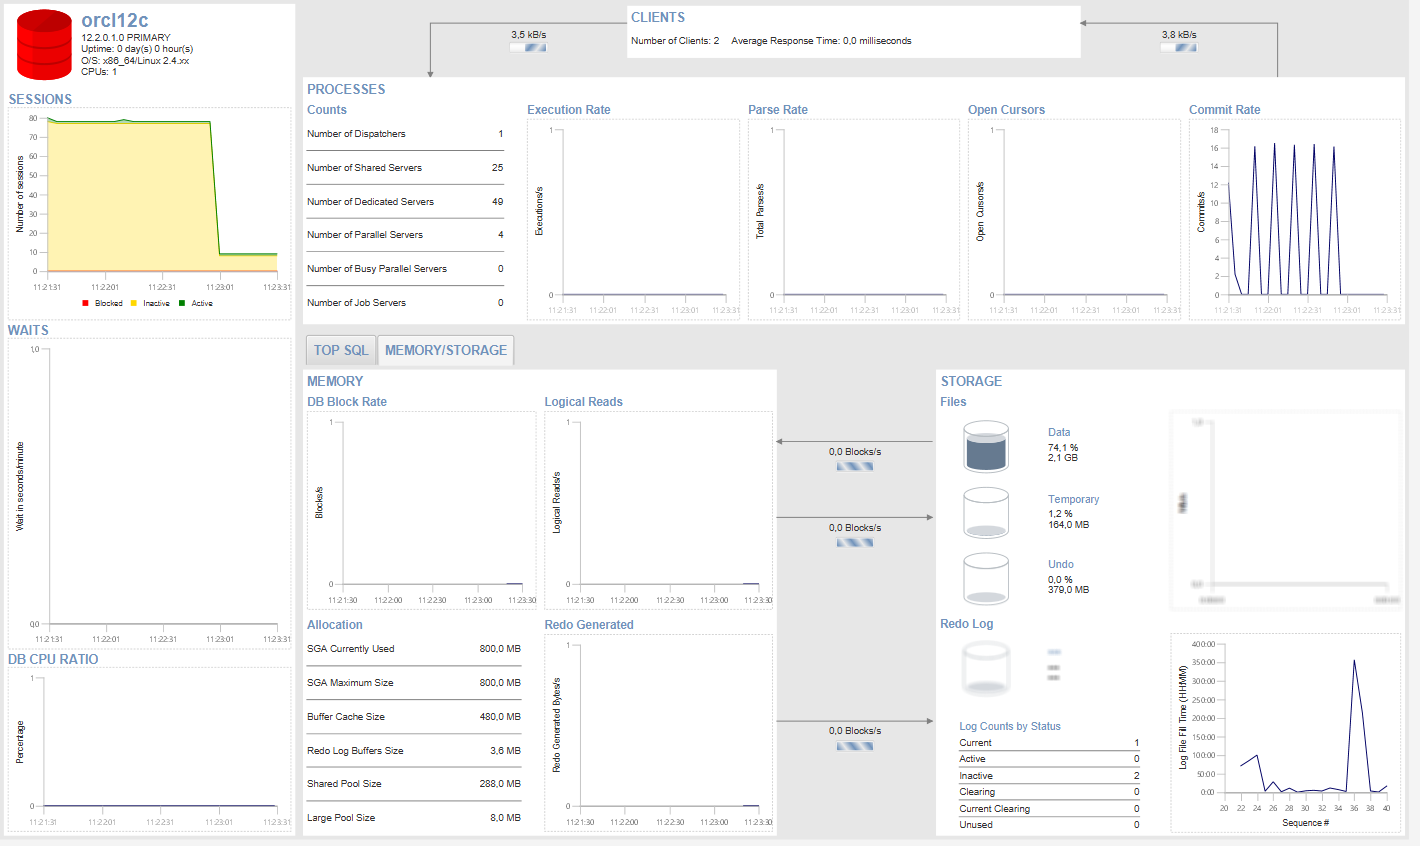
\includegraphics[scale=0.45]{html/sqldev.png}
\caption{\emph{Instance Viewer} - monitor do SQLDeveloper, apresentando o momento final de transição antes/depois do uso do \emph{swingbench}. Pode-se observar. pelo gráfico de número de sessões no canto superior esquerdo, que há uma descida abrupta de número de sessões.}
\end{figure}

\begin{figure}[H]
\centering
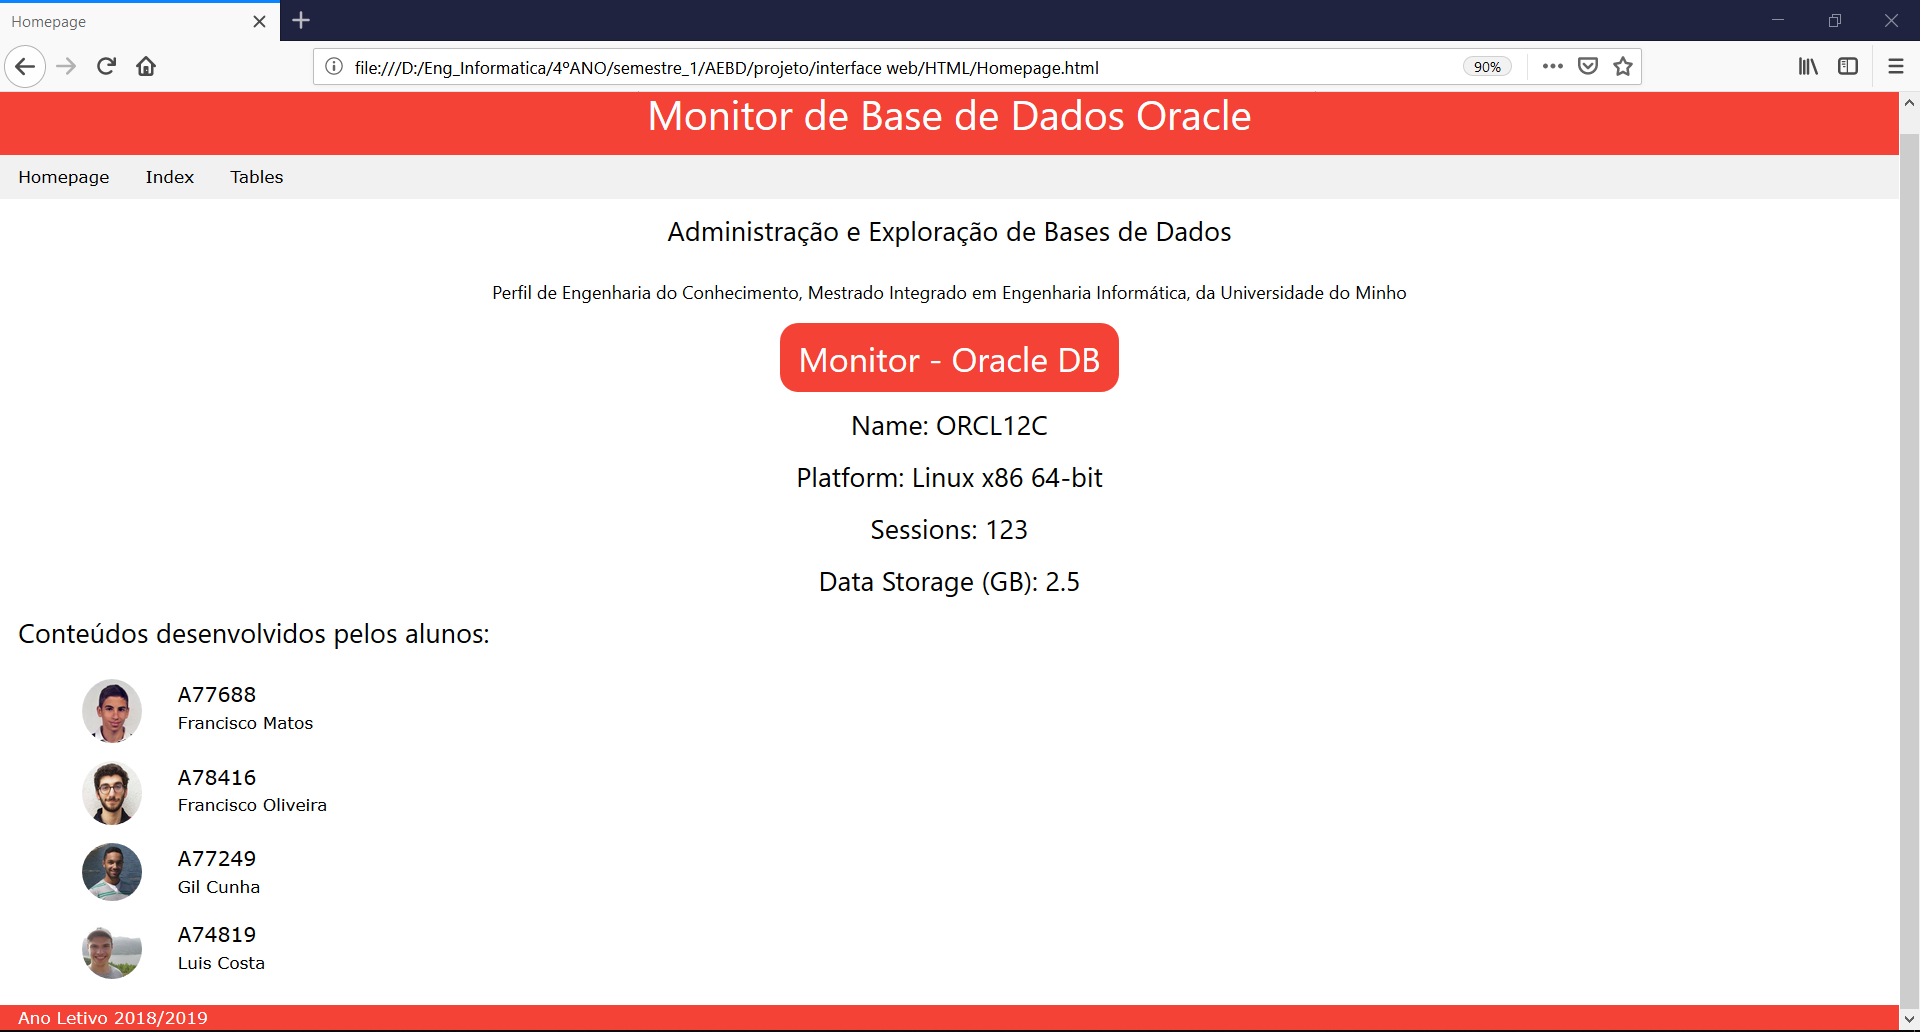
\includegraphics[scale=0.4]{html/homepage.png}
\caption{\emph{Homepage} da interface \emph{web}, onde são apresentados os elementos do grupo e as informações gerais da base de dados \emph{pluggable}, como o seu nome, plataforma da máquina que a contem, número de sessões e \emph{data storage}.}
\end{figure}

\begin{figure}[H]
\centering
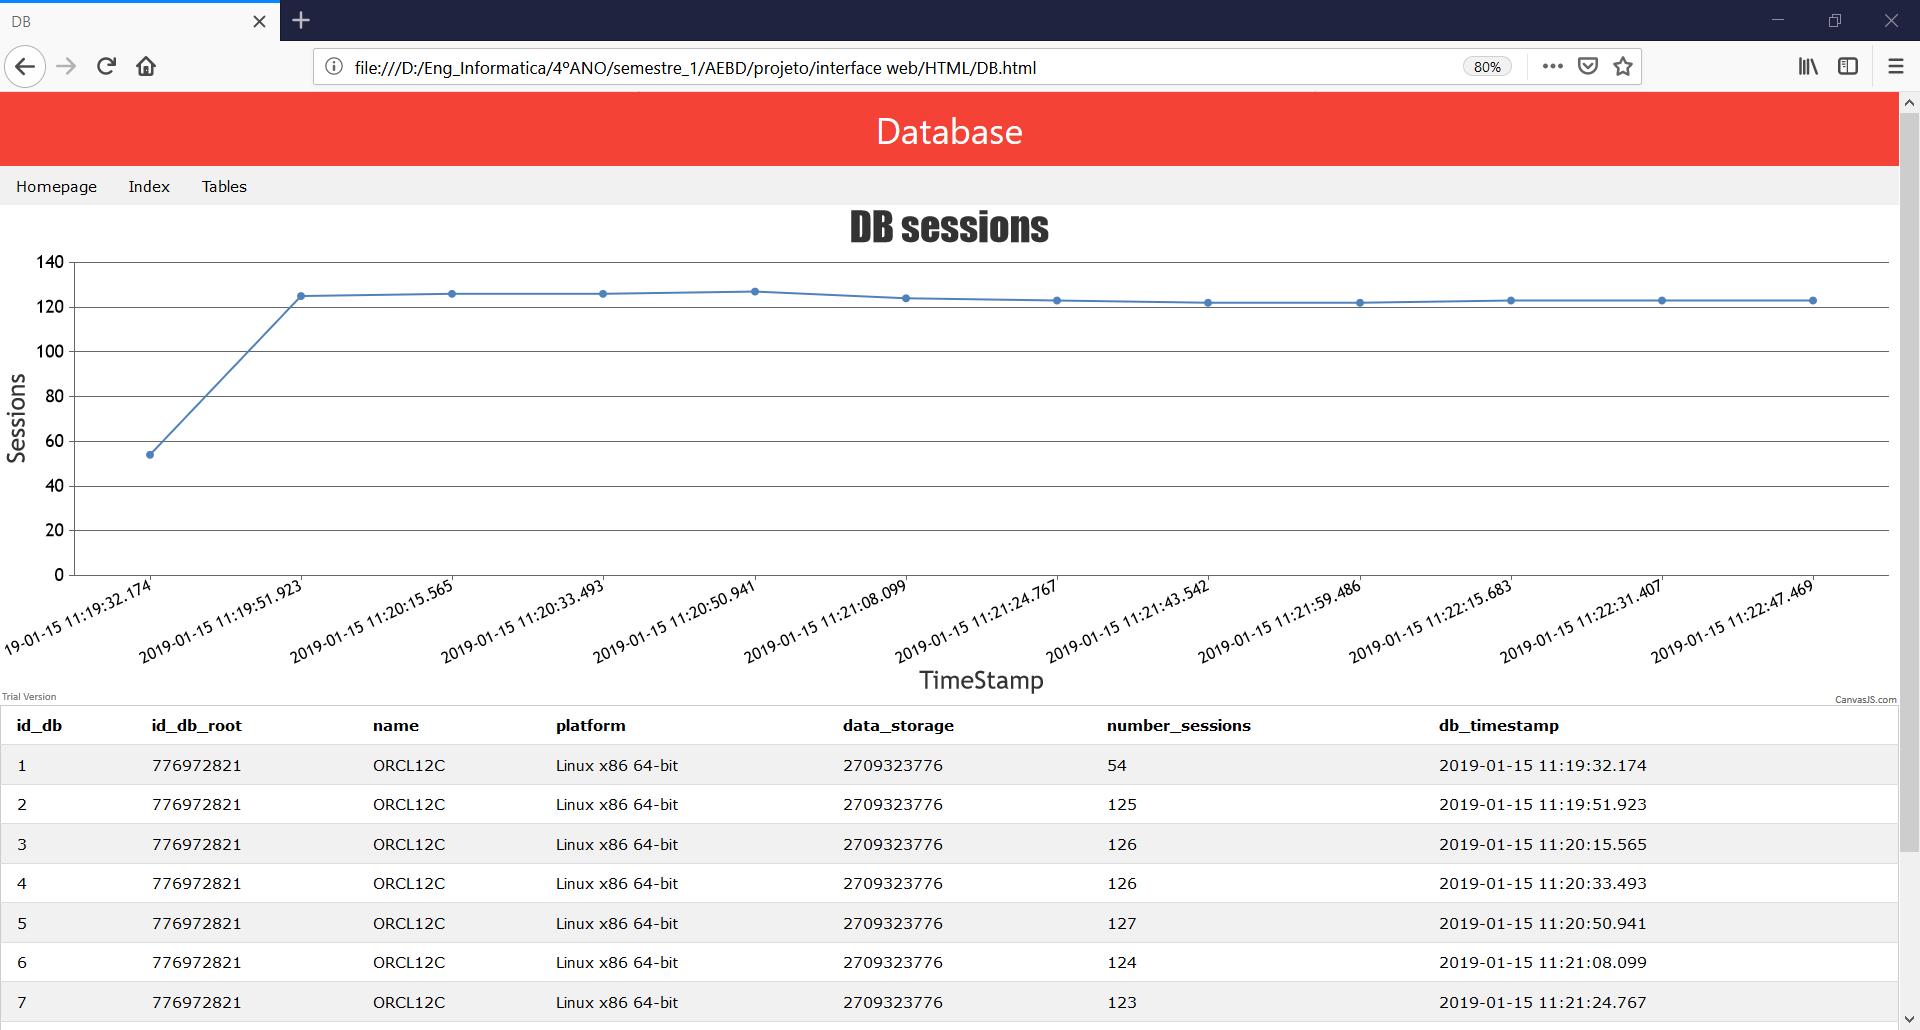
\includegraphics[scale=0.4]{html/db.png}
\caption{Página que apresenta a informação recolhida sobre a Base de Dados \emph{pluggable}, que contem um gráfico "de linha" sobre o número de sessões ao longo do tempo (histórico de nº de sessões) e a tabela com os dados obtidos nos vários ciclos de recolha.}
\end{figure}

\begin{figure}[H]
\centering
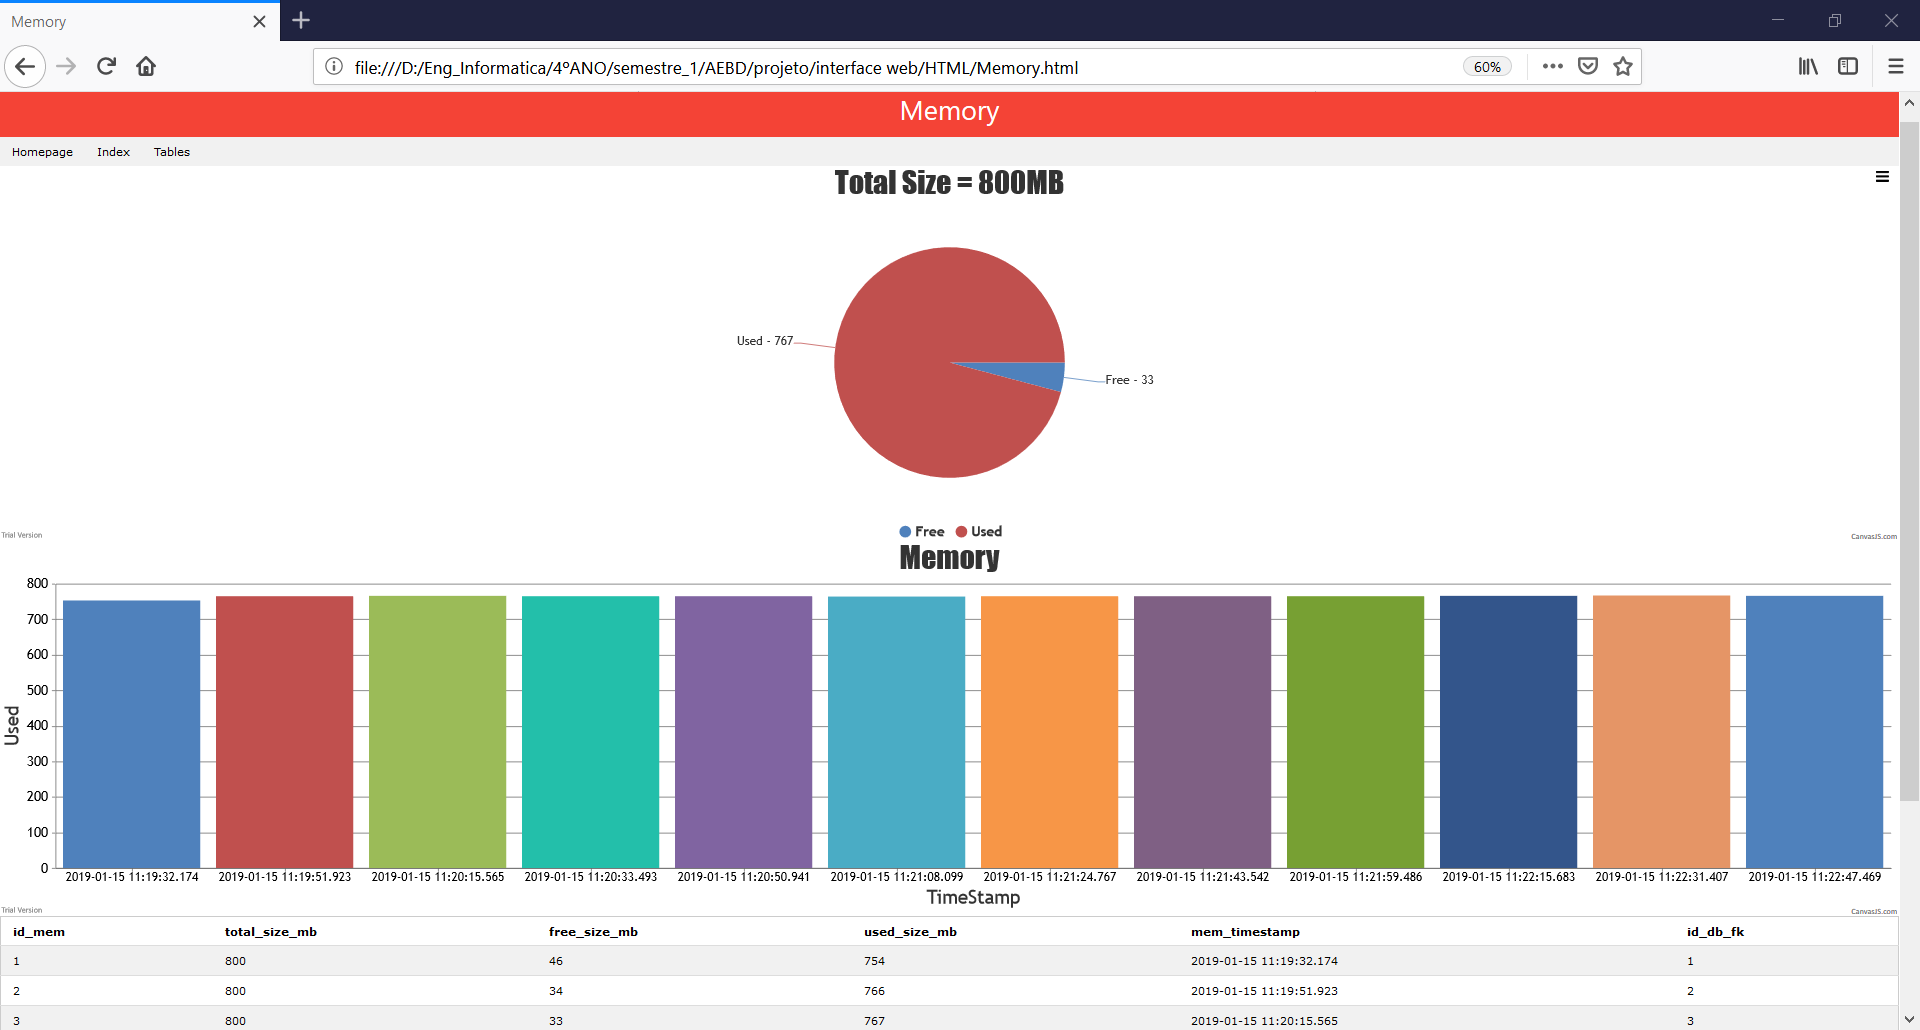
\includegraphics[scale=0.4]{html/mem.png}
\caption{Página que apresenta a informação recolhida sobre a memória da Base de Dados \emph{pluggable}, que contem um gráfico circular a relação entre o espaço de memória disponível e utilizado, no momento atual, um gráfico de barras com o espaço de memória utilizado ao longo do tempo (histórico de memória utilizada) e a tabela com os dados obtidos nos vários ciclos de recolha.}
\end{figure}

\begin{figure}[H]
\centering
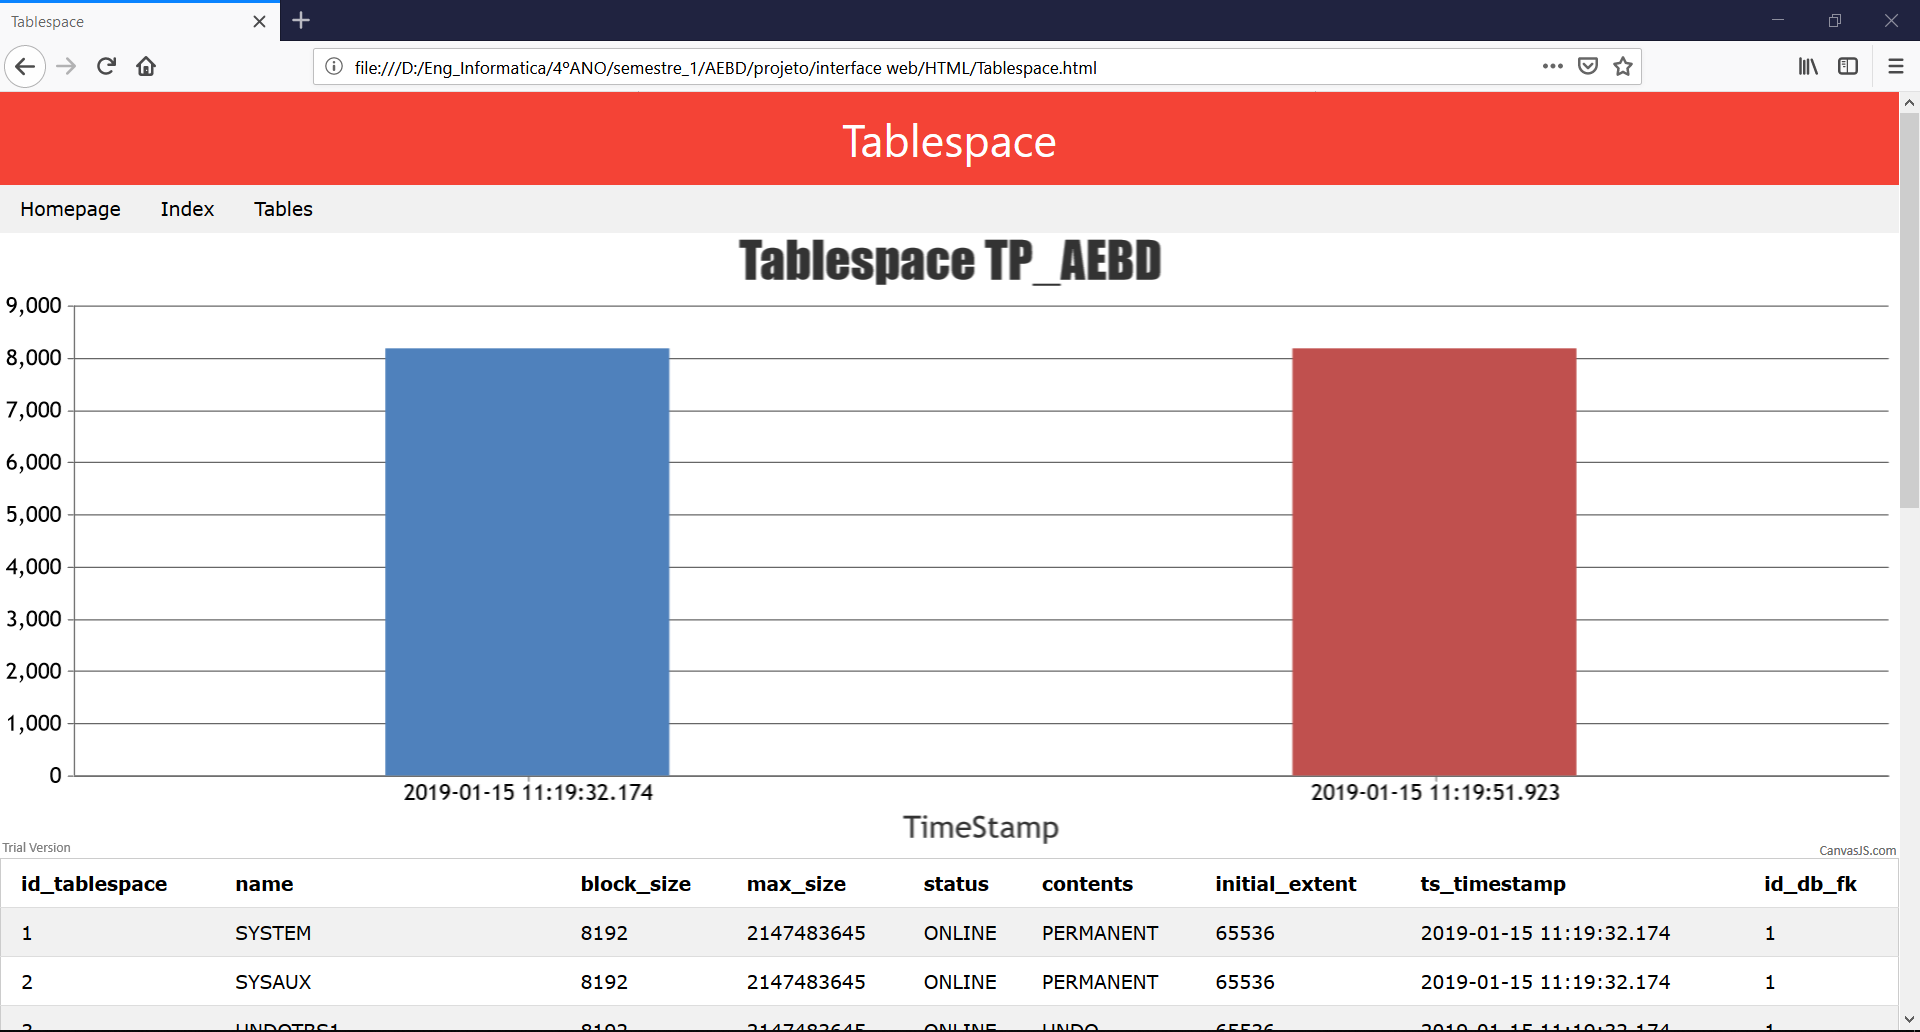
\includegraphics[scale=0.4]{html/tablespace.png}
\caption{Página que apresenta a informação recolhida sobre a \emph{tablespace} TP\_AEBD, que contem um gráfico de barras com o espaço de ocupado por esta ao longo do tempo (histórico de memória utilizada) e a tabela com os dados obtidos nos vários ciclos de recolha}
\end{figure}

\newpage
\section{Conclusão}
\hspace{3mm} 

A criação de um monitor capaz de supervisionar o desempenho de uma Base de Dados (\emph{pluggable}), permitiu-nos verificar o peso que certas operações podem ter na utilização das mesmas. 

Na realização do sistema do projeto apresentaram-se algumas dificuldades, tais como: o planeamento da estrutura capaz de armazenar corretamente a informação pretendida, a seleção dos parâmetros para análise da performance da \emph{pluggable} DB e a seleção da linguagem de programação para a criação do agente responsável por monitorizar a \emph{pluggable} DB. Porém o grupo considera que as superou por completo e concluiu o projeto com sucesso, visto ter alcançado todos os objetivos.

Ainda de referir que, na representação dos dados obtidos, foi tido em atenção a necessidade que a interface criada fosse \emph{user-friendly}, isto é, uma interface intuitiva e de fácil interpretação para qualquer utilizador.

Em suma, com este trabalho prático, o conhecimento e compreensão dos elementos do grupo sobre o funcionamento geral de uma base da dados \emph{Oracle} e as suas estruturas, desenvolveram-se bastante. Foi, assim, um projeto muito produtivo e positivo.

\end{document}